


%%%%%%%%%%%%%%%%%%%%%%%%%%%%%%%%%%%%%%%%%%%%%%%%%%%%%%%%%%%%%
%% HEADER
%%%%%%%%%%%%%%%%%%%%%%%%%%%%%%%%%%%%%%%%%%%%%%%%%%%%%%%%%%%%%
\documentclass[a4paper,twoside,11pt]{report}
\usepackage{a4}

\title{Entwicklung und Fertigung eines selbstfahrenden Modellautos}
\author{Felix Sandri, Philipp Kaltenleitner, Mert Guerel, David Petrovic}

\usepackage[text={150mm,240mm},bindingoffset=1cm]{geometry}

%% Deutsche Anpassungen %%%%%%%%%%%%%%%%%%%%%%%%%%%%%%%%%%%%%
\usepackage[ngerman]{babel}
\usepackage[T1]{fontenc}
\usepackage[ansinew]{inputenc}

\usepackage{lmodern} %Type1-Schriftart f�r nicht-englische Texte
\usepackage{color}
\usepackage{xcolor}

\usepackage{array} %F�r die Eidesstattliche Erkl�rung
\usepackage{float} %Fliegende Abbildungen / Objekte
\usepackage[margin=10pt,labelfont=bf,singlelinecheck=false]{caption}

\usepackage{hyperref}	%Querverweise
\usepackage{inputenc} 

\usepackage{fancyhdr} %Kopf- und Fu�zeile
\usepackage{lastpage} %letzte Seite referenzierbar
\usepackage{scrlayer}	%Page-Styles

%% Packages f�r Grafiken & Abbildungen %%%%%%%%%%%%%%%%%%%%%%
\usepackage{graphicx} %Zum Laden von Grafiken

%% Packages f�r Formeln %%%%%%%%%%%%%%%%%%%%%%%%%%%%%%%%%%%%%
\usepackage{amsmath}
\usepackage{amsthm}
\usepackage{amsfonts}



%%%%%%%%%%%%%%%%%%%%%%%%%%%%%%%%%%%%%%%%%%%%%%%%%%%%%%%%%%%%%
%% DOKUMENT
%%%%%%%%%%%%%%%%%%%%%%%%%%%%%%%%%%%%%%%%%%%%%%%%%%%%%%%%%%%%%
\begin{document}

\pagestyle{empty} %%Keine Kopf-/Fusszeilen auf den ersten Seiten.

%% Deckblatt %%%%%%%%%%%%%%%%%%%%%%%%%%%%%%%%%%%%%%%%%%%%%%%%
% Beginn - Formatierung der Titelseite

\vspace*{3pt}
\parbox[c]{80mm}{
	\begin{Large}\textbf{HTBLuVA Salzburg }\end{Large} \newline
	\textbf{H�here Lehranstalt f�r Elektrotechnik} \newline
	Ausbildungsschwerpunkt: \newline Energiesysteme und Industrieelektronik
}
\hfill
\parbox[c]{60mm}{  
	
\includegraphics[width=\linewidth]{./Abbildungen/HTBLuVA_Salzburg_Logo_RGB.jpg}
}
\hrule\relax

\vspace*{30mm}
\begin{center} 
\begin{Huge}\textbf{Diplomarbeit}\end{Huge} \par \bigskip 
\begin{Large}5BHET 2023/24 \par \bigskip 
H�here Technische Bundeslehr- und Versuchsanstalt Salzburg \par \bigskip 
Abteilung f�r Elektrotechnik\end{Large} 
\vspace*{20mm}

%		In der Hautpdatei nach \usepackage{a4} folgendes Einf�gen:
%		\title{Entwicklung einer Diplomarbeitsvorlage}

\begin{huge}
	\makeatletter
	\textbf{\@title \\[1ex]}
	\makeatother
\end{huge}
\end{center}

\vspace{3cm}
\parbox[c]{60mm}{%
	\textbf{Ausgef�hrt von:}\par
	Felix Sandri\\
	Philipp Kaltenleitner\\	
	Mert G�rel\\
	David Petrovic\\
}%
\hfill%
\parbox[c]{70mm}{%
	\textbf{Betreuer}:\par
	BSc Simon Dantendorfer\\
	Prof. Dipl.-Ing. Reinhold Benedikter\\
	Prof. Dipl.-Ing. Robert Fuchs\\
	Prof. Dipl.-Ing. Timo Huemer\\
}%

\newpage
% Ende - Formatierung der Titelseite 

%% Eidesstattliche Erkl�rung %%%%%%%%%%%%%%%%%%%%%%%%%%%%%%%%
\newpage
\pagestyle{plain}
\pagenumbering{Roman}
\vspace*{0cm}
\begin{center}
\textbf{\Huge{Eidesstattliche Erkl�rung}}
\end{center}
\vspace{1cm}

Wir erkl�ren an Eides statt, dass wir die vorliegende Arbeit selbstst�ndig und ohne fremde Hilfe verfasst, andere als die angegebenen Quellen nicht benutzt und die den benutzten Quellen w�rtlich und inhaltlich entnommenen Stellen als solche kenntlich gemacht haben.\\
Wir versichern, dass wir dieses Diplomarbeitsthema bisher weder im In- noch im Ausland (einer Beurteilerin oder einem Beurteiler) in irgendeiner Form als Pr�fungsarbeit vorgelegt haben.



%\vspace*{3cm}
%\begin{tabular}{p{4cm}p{5cm}p{4cm}}
%\hrulefill & & \hrulefill \\ 
%\centering Jakob Buchsteiner & & \centering Thomas Eibl \\
%\hrulefill & & \hrulefill \\
%\hrulefill & & \hrulefill \\ 
%\centering Sebastian Neuhofer & & \centering Moritz Taferner
%\end{tabular}

% \usepackage{array} is required
\vspace*{3cm}
\begin{center}
\begin{tabular}{
	>{\centering\arraybackslash}p{4cm}
	>{\centering\arraybackslash}p{4cm}
	>{\centering\arraybackslash}p{4cm}}
            \hrulefill         &  & \hrulefill      \\
            Felix Sandri       &  & Philipp Kaltenleitner     \vspace*{1.5cm}\\ 
            \hrulefill         &  & \hrulefill      \\
            Mert G�rel         &  & David Petrovic            \vspace*{2cm}\\
            & \hrulefill & \\
            & Ort, Datum & \\
\end{tabular} 
\end{center}
	

%% Vorwort %%%%%%%%%%%%%%%%%%%%%%%%%%%%%%%%%%%%%%%%%%%%%%%%%%
\newpage
\chapter*{Vorwort}
	TEST \cite{Kaltenleitner2019}

%% Abstract %%%%%%%%%%%%%%%%%%%%%%%%%%%%%%%%%%%%%%%%%%%%%%%%%
\newpage
\textbf{\Huge{Diplomarbeitsdokumentation}}

\begin{tabular}{|m{4.5cm}|m{9cm}|}															%senkrechter Strich steht f�r horizontale Linien
																																%mit m k�nnen die Gr��en der Zellen bestimmt werden
		\hline																											% \hline f�r eine horizontale Linie in der Tabelle
		& \\																												% mit & werden die Zellen abgerentzt
		Verfasser & Felix Sandri, Philipp Kaltenleitner, \\	% \\ steht f�r einen Zeilenumbruch in einer Tabelle
							& Mert G�rel, David Petrovic  \\ 
		& \\				
		\hline
		& \\
		Jahrgang Schuljahr & 5BHET \\ & 2023/24  \\ 								
		& \\ 			
		\hline
		
		& \\
		Thema der & Entwicklung und Fertigung eines selbstfahrenden \\ 
		Diplomarbeit & Modelautos\\ 
		& \\ 
		\hline
		& \\
		Kooperationspartner & HTBLuVA Salzburg \\ 
												& Kyocera AVX \\
											  & Mean Well/ Pro Connect \\ 
												& WG Global GmbH\\
												& SDP Automobile\\	
												& Mario's Autoteile\\	
												& Innovation Salzburg Pioniergarage GmbH\\ 
												& Schraubenking GmbH\\	
												
		& \\
		\hline \hline
		
		& \\
		Aufgabenstellung & Das Ziel besteht darin, ein Modellauto zu entwickeln, welches auf dem Gel�nde der HTBLuVA Salzburg autonom fahren kann. Hierf�r wird ein Auto von Grund auf neu konstruiert, inklusive aller mechanischen, elektronischen und softwaretechnischen Komponenten. Des Weiteren soll das Fahrzeug in allen mechanischen und elektrotechnischen Aspekten voll funktionsf�hig sein.
		\\
		& \\ 
		\hline \hline
		& \\
		
		Realisierung & Um das autonome Fahren zu erm�glichen, wird ein vollst�ndig neues Fahrzeug mit allen erforderlichen mechanischen Komponenten entwickelt, das ausreichend Platz bietet, um s�mtliche Elektronik unterzubringen. Zur Umgebungserfassung nutzt Athena einen LiDAR-Sensor sowie acht weitere Ultraschallsensoren. Die Hauptrecheneinheit ist ein Lattepanda 3 Delta, der zudem �ber eine Dual Edge TPU verf�gt, was eine schnellere Verarbeitung der Sensordaten erm�glicht. Durch k�nstliche Intelligenz kann Athena nicht nur die Daten verarbeiten, sondern auch das Fahrzeug steuern. Zus�tzlich wird ein ESP32 als Sub-Prozessor verwendet.\\
		 
		& \\ 
		\hline
		
		\end{tabular}	
		
		\pagebreak
				
		\begin{tabular}{|m{4.5cm}|m{9cm}|}
		
		\hline
		& \\
		Abbildung & 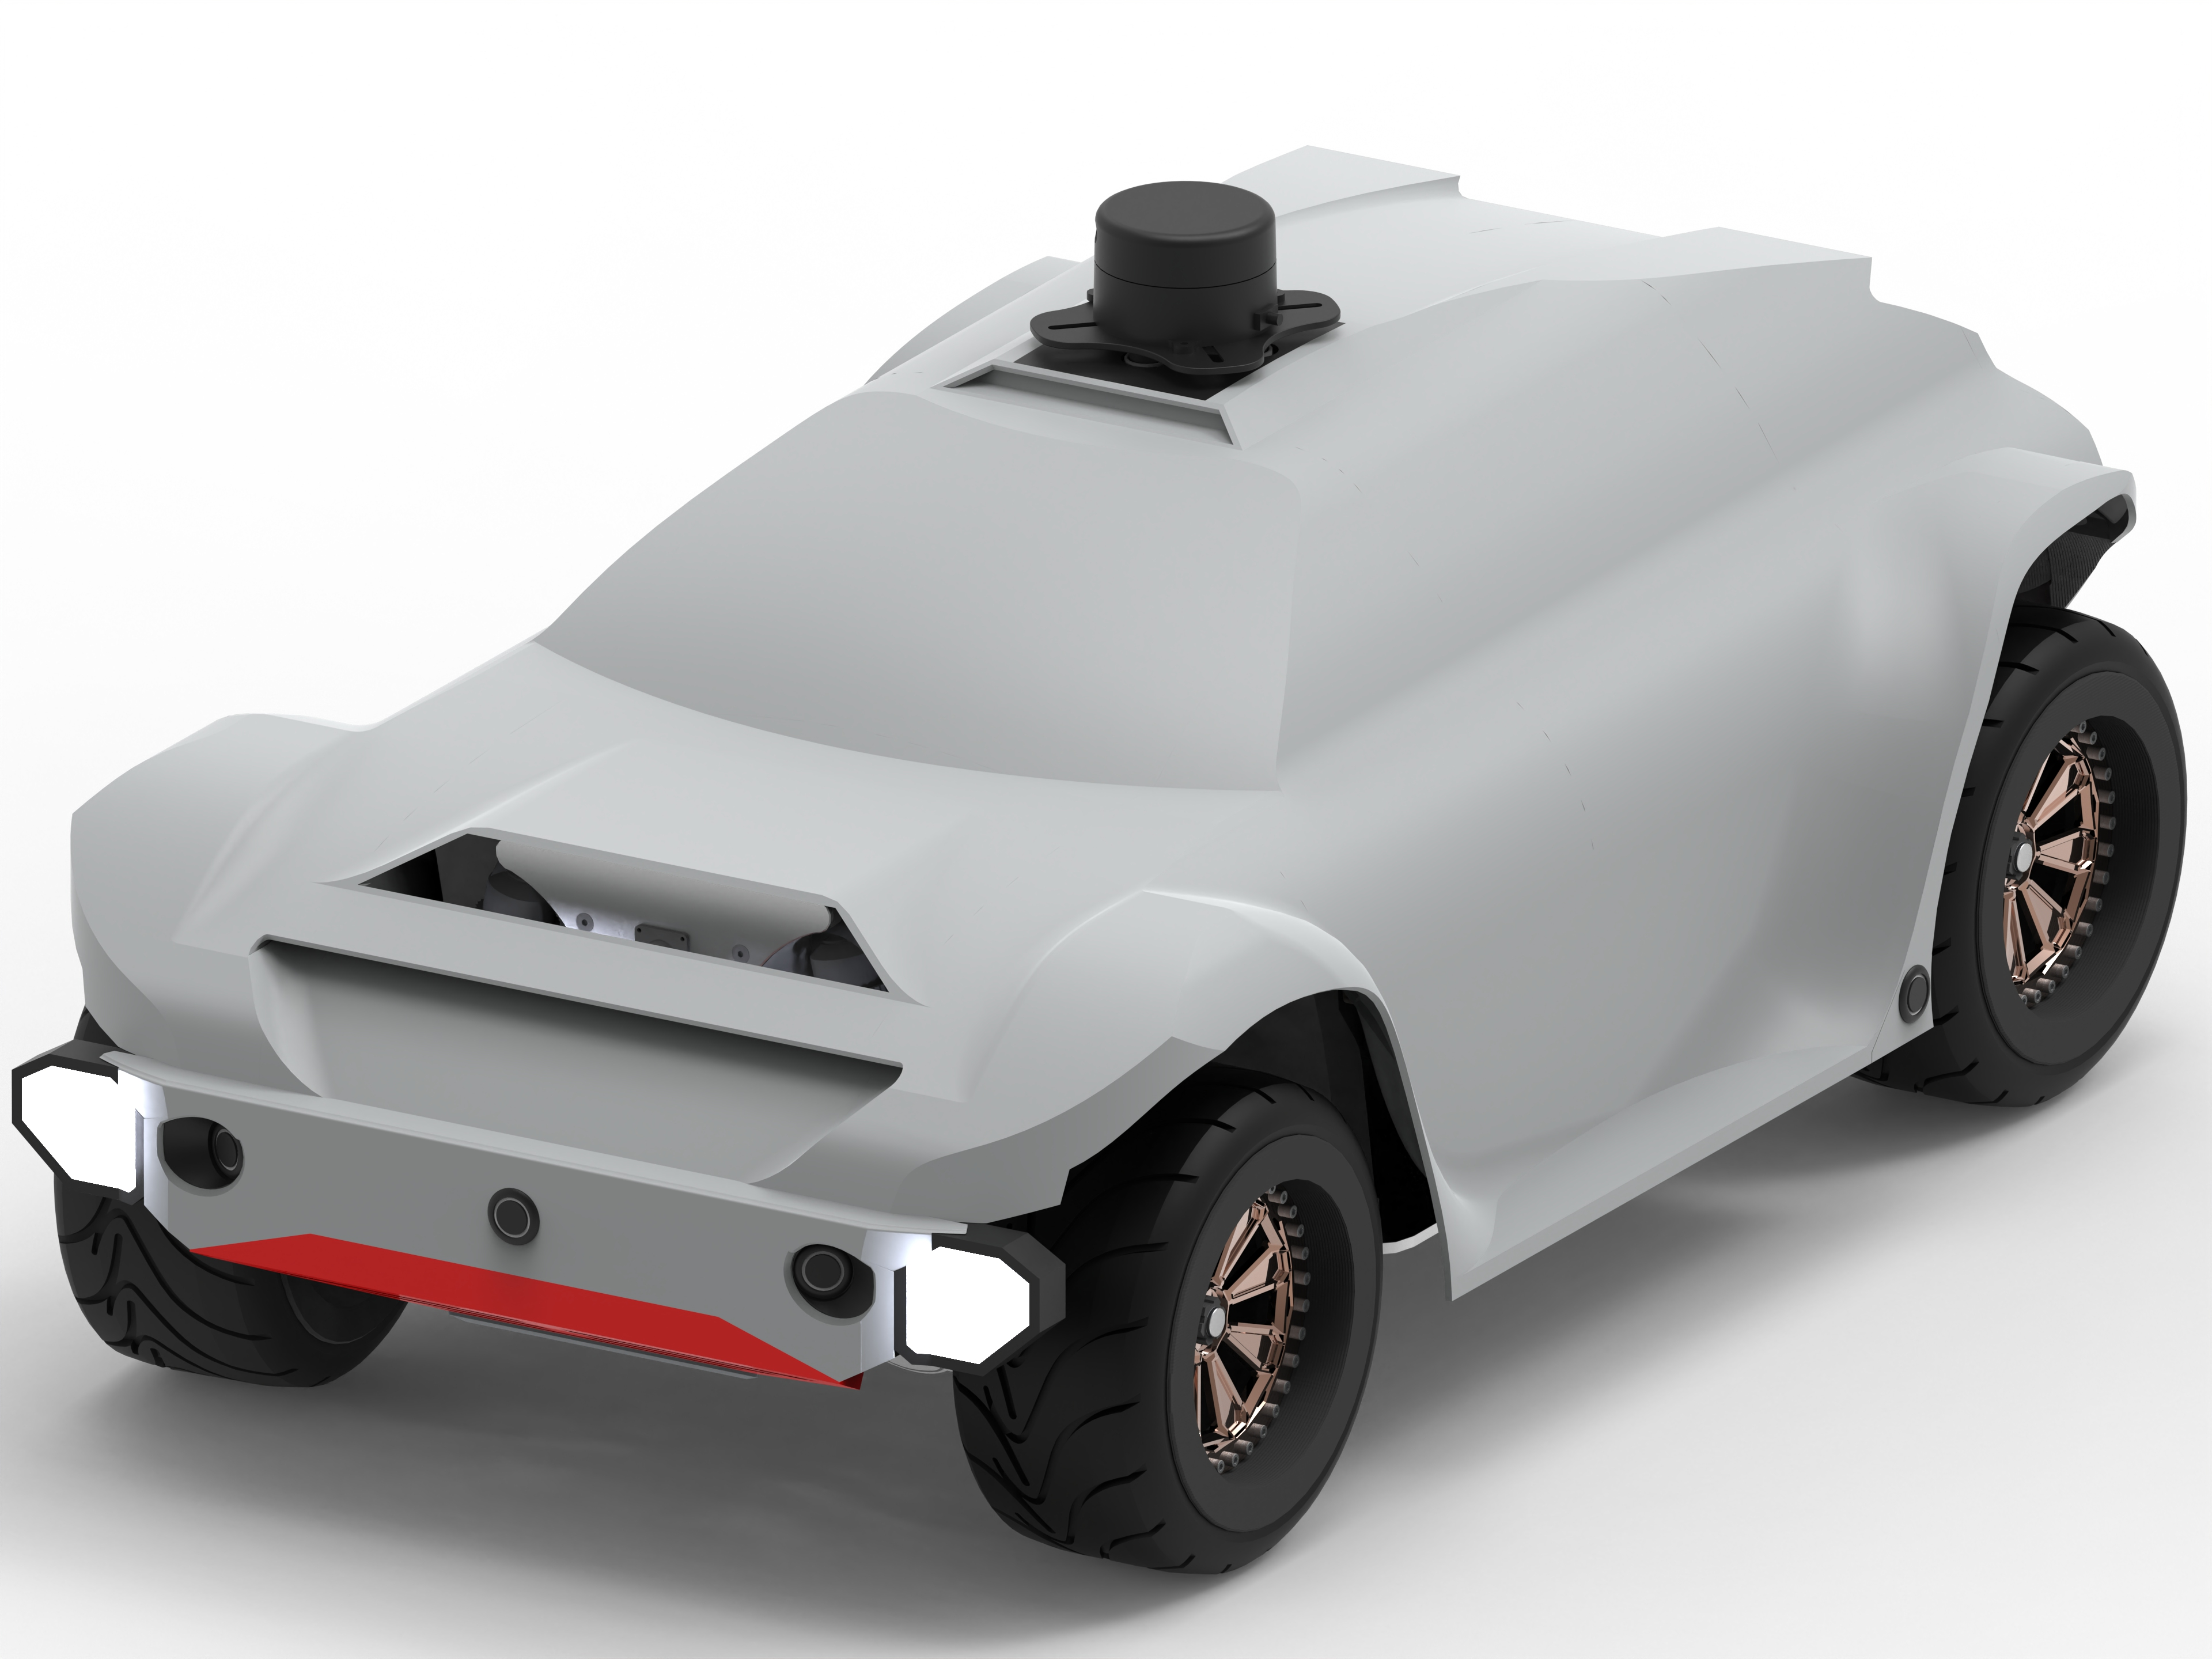
\includegraphics[width=8.5cm]{./4_Mechanik/Abbildungen/Aufbau_Anleitung_render/Athena_fertig_4}\\ 
		& \\
		\hline 
	
		\end{tabular}	
		
		\begin{tabular}{|m{4.5cm}|m{9cm}|}
		
		\hline
		Ergebnisse & Das Modellauto Athena wurde sowohl mechanisch als auch in Bezug auf Hardware und Software rechtzeitig fertiggestellt und erfolgreich in Betrieb genommen. \\ 
		\hline
		
		\end{tabular}
		
		\begin{tabular}{|m{4.5cm}|m{9cm}|}\hline
		
		M�glichkeit der Einsichtnahme in die Arbeit & Die Diplomarbeit ist in gebundener Form in der
																									Schulbibliothek als auch bei AV Prof. Dipl-Ing.
																									(FH) Roland Holzer einzusehen. Dar�ber hinaus besitzt
																									jedes Mitglied des Projektteams eine vollst�ndige Version 
																									in gebundener und digitaler Form. \\ 
		\hline  
		
		\end{tabular}
		
		\begin{tabular}{|m{4.5cm}|m{4.28cm}|m{4.28cm}|}	%letzte Zeile muss in 3 Spalten unterteilt werden
		
		\hline
		
		Approbation & Pr�fer/Pr�ferin & Abteilungsvorstand \\ 
		(Datum/Unterschrift) &  & 	\\  
		&	& \\ 
		\hline

		\end{tabular}					%Ende der Tabelle
		\newpage
		
		
		
		
		
		
		
		\textbf{\Huge{Diploma Thesis Documentation}}

\begin{tabular}{|m{4.5cm}|m{9cm}|}															%senkrechter Strich steht f�r horizontale Linien
																																%mit m k�nnen die Gr��en der Zellen bestimmt werden
		\hline																											% \hline f�r eine horizontale Linie in der Tabelle
		& \\																												% mit & werden die Zellen abgerentzt
		Authors & Felix Sandri, Philipp Kaltenleitner, \\	% \\ steht f�r einen Zeilenumbruch in einer Tabelle
							& Mert G�rel, David Petrovic  \\
		& \\				
		\hline
		& \\
		Form Academic year & 5BHET \\ & 2023/24  \\ 								
		& \\ 			
		\hline
		
		& \\
		Topic & Development and Manufacturing of a Self-Driving\\ 
					& Model Car\\ 
		& \\ 
		
		\hline
		
		& \\
		Co-operation  			& HTBLuVA Salzburg \\ 
												& Kyocera AVX \\
											  & Mean Well/ Pro Connect \\ 
												& WG Global GmbH\\
												& SDP Automobile\\	
												& Mario's Autoteile\\	
												& Innovation Salzburg Pioniergarage GmbH\\ 
												& Schraubenking GmbH\\	
												
		& \\
		\hline \hline
		& \\
	Assignment of Tasks & The goal is to develop a model car capable of autonomous driving on the premises of HTBLuVA Salzburg. To achieve this, a car will be completely designed from scratch, including all mechanical, electronic, and software components. Furthermore, the vehicle is intended to be fully functional in all mechanical and electrical aspects. \\
		& \\ 
		\hline \hline
		& \\
		 
		Realization & To enable autonomous driving, a completely new vehicle is being developed with all necessary mechanical components, providing ample space to accommodate all electronics. Athena utilizes a LiDAR sensor and eight additional ultrasonic sensors for environment mapping. The main computing unit is a Lattepanda 3 Delta, equipped with a Dual Edge TPU for faster sensor data processing. Through artificial intelligence, Athena can not only process data but also control the vehicle. Additionally, an ESP32 is used as a sub-processor. \\
		 
		& \\ 
		\hline
		
		\end{tabular}	
		
		\begin{tabular}{|m{4.5cm}|m{9cm}|}
		
		\hline
		
		& \\
		Illustrative Graph & 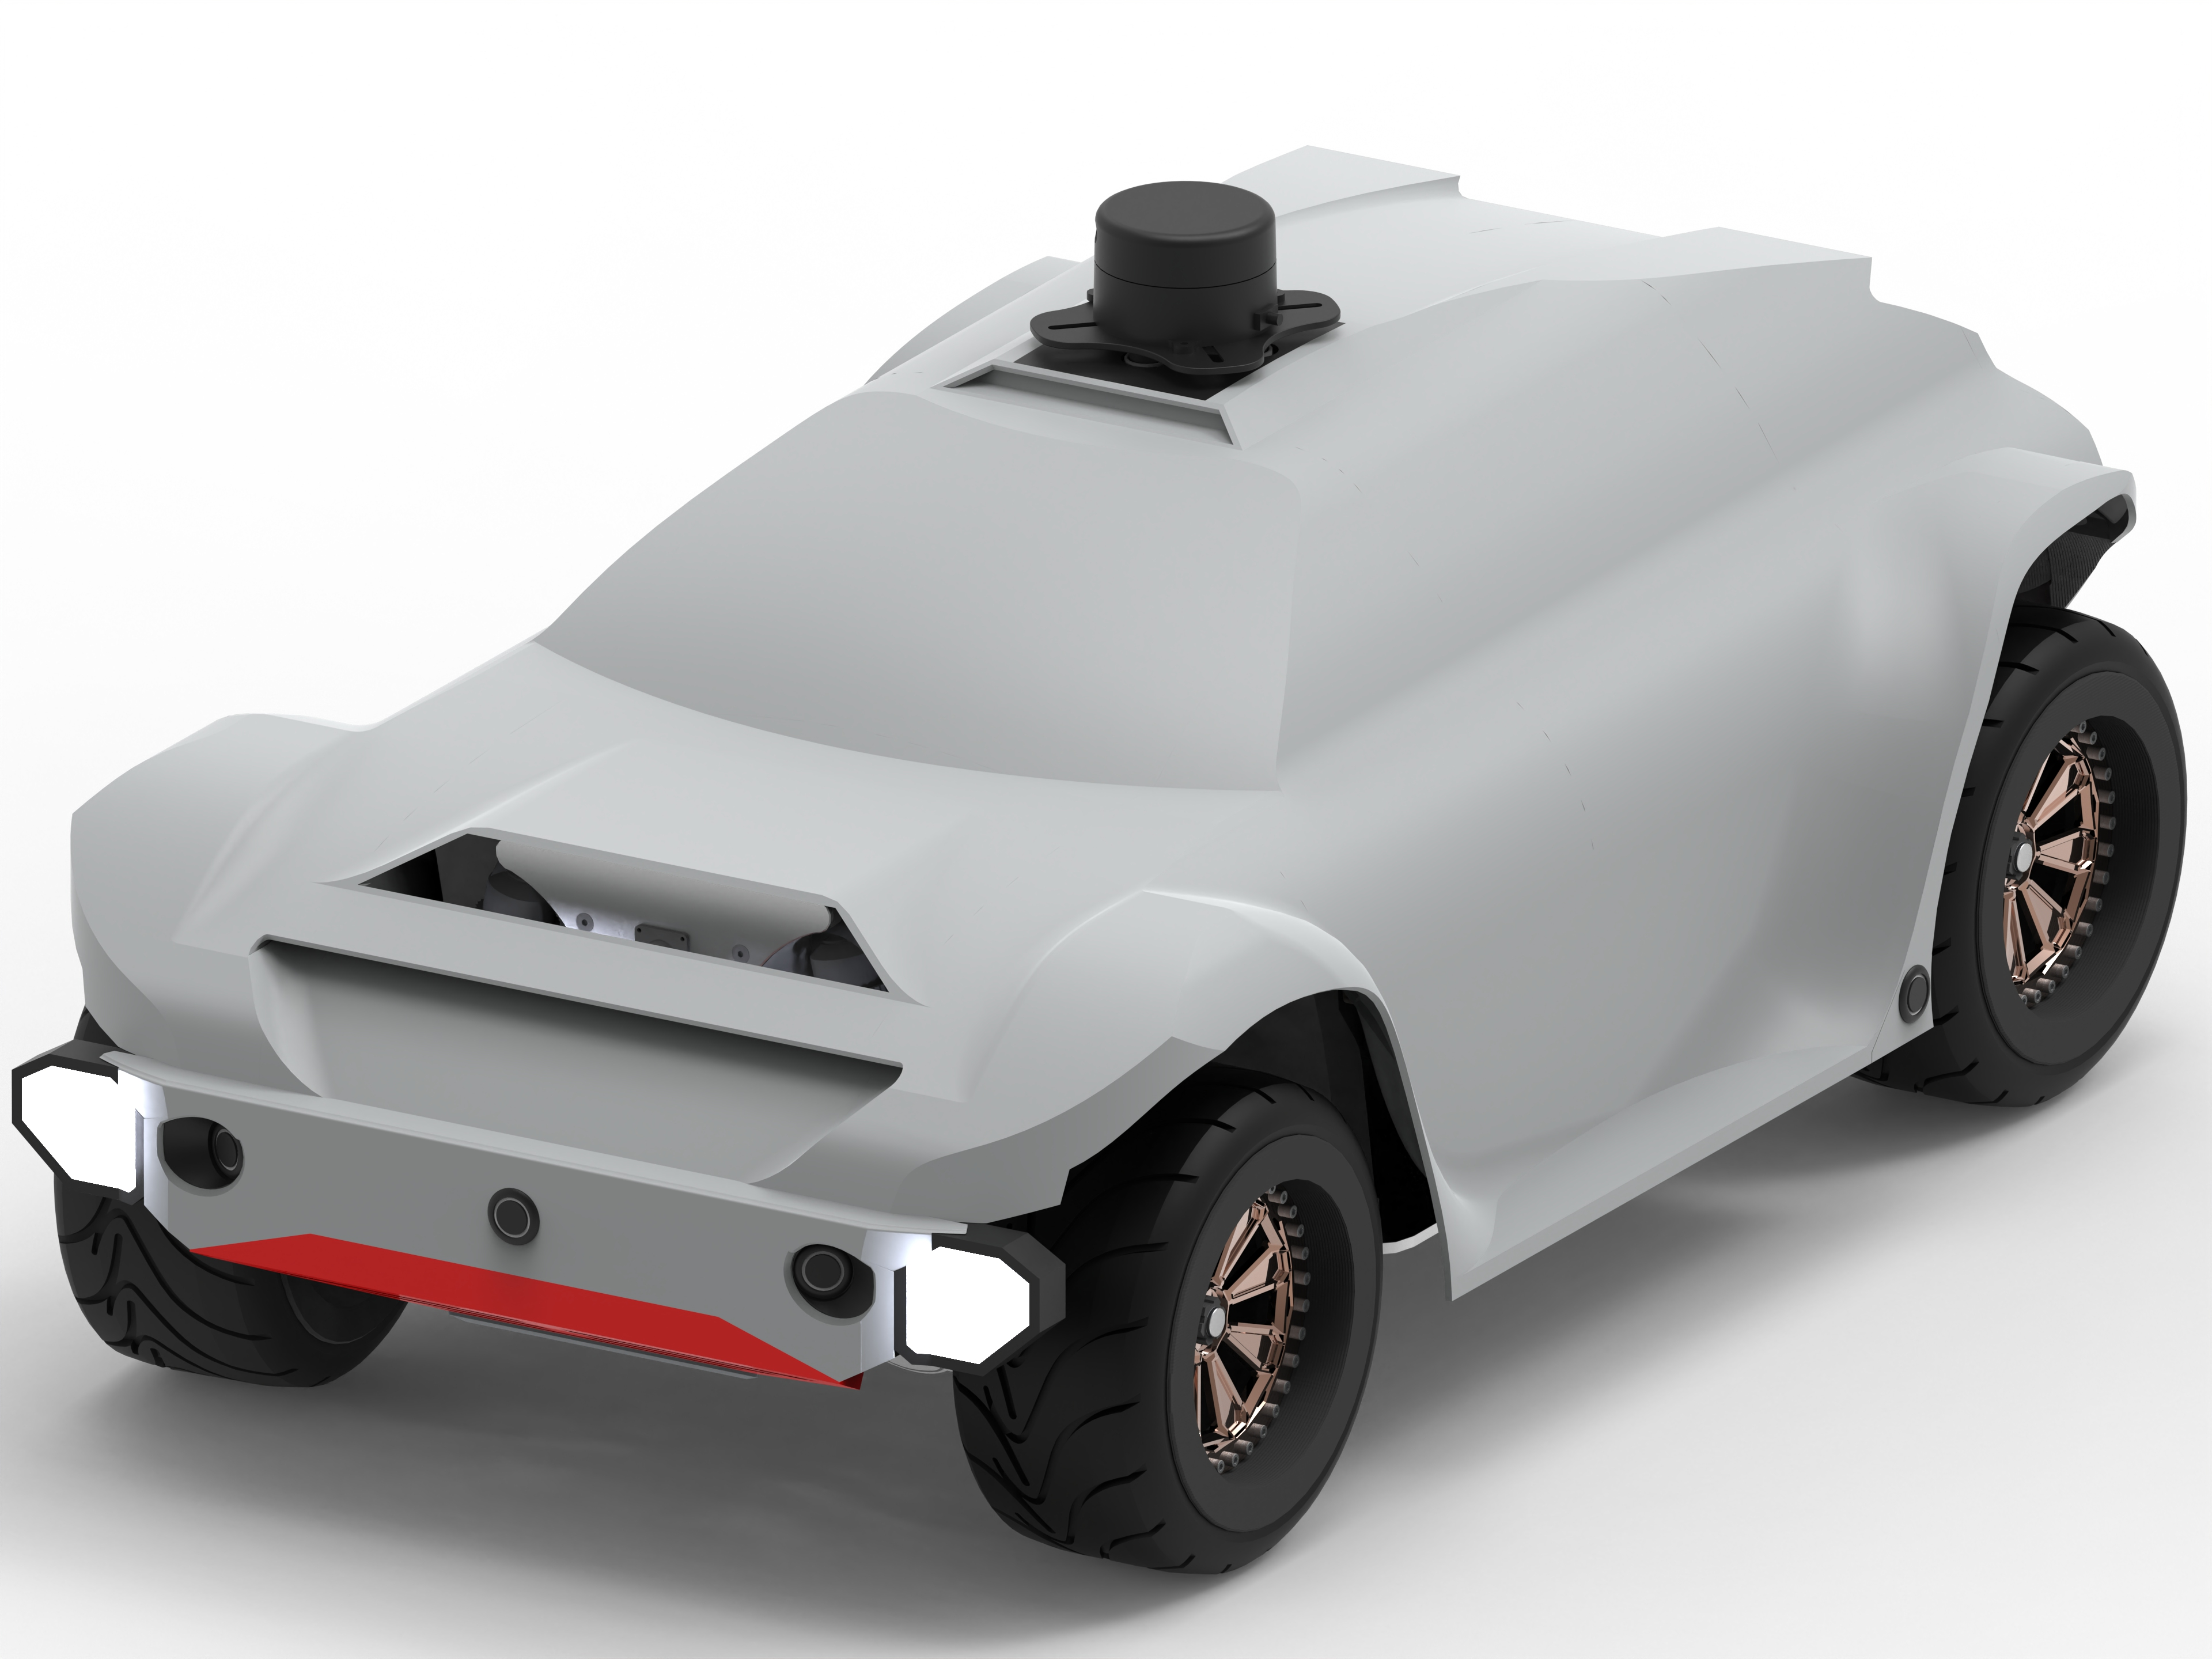
\includegraphics[width=8.5cm]{./4_Mechanik/Abbildungen/Aufbau_Anleitung_render/Athena_fertig_4}\\ 
		& \\
		
		\hline 
	
		\end{tabular}	
		
		\begin{tabular}{|m{4.5cm}|m{9cm}|}
		
		\hline
		Results & The model car Athena has been completed on time, both mechanically and in terms of hardware and software, and has been successfully put into operation. \\ 
		\hline
		
		\end{tabular}
		
		\begin{tabular}{|m{4.5cm}|m{9cm}|}\hline
		
		Accessibility of \newline Diploma Thesis	 		& 		The diploma thesis is available in the school library
																												as well as in the office of the head of department
																												Prof. Dipl-Ing. (FH) Roland Holzer. In addition,
																												each member of the project team has a complete
																												version in hardcover and digital form.\\ \hline  
		
		\end{tabular}
		
		\begin{tabular}{|m{4.5cm}|m{4.28cm}|m{4.28cm}|}	%letzte Zeile muss in 3 Spalten unterteilt werden
		
		\hline
		Approval & Examiner & Head of department \\ 
		(Date/Sign) &  & 	\\  
		& & \\ 
		\hline
		\end{tabular}					%Ende der Tabelle
		\newpage

%% Inhaltsverzeichnis %%%%%%%%%%%%%%%%%%%%%%%%%%%%%%%%%%%%%%%
\tableofcontents %Inhaltsverzeichnis
\cleardoublepage %Das erste Kapitel soll auf einer ungeraden Seite beginnen.

\pagestyle{plain} %%Ab hier die Kopf-/Fusszeilen: headings / fancy / .
\pagenumbering{arabic}

%% Einf�hrung %%%%%%%%%%%%%%%%%%%%%%%%%%%%%%%%%%%%%%%%%%%%%%%
\newpage
\chapter{Einf�hrung}
	
	\section{Projektteam}
	
	\section{Projektbetreuer}
		\begin{itemize}
			\item \textbf{Prof. Dipl.-Ing. Robert Fuchs}
			\item \textbf{Prof. Dipl.-Ing. Reinhold Benedikter}
			\item \textbf{BSc Simon Dantendorfer}
			\item \textbf{Prof. Dipl.-Ing. Timo Huemer}
		\end{itemize}
	
	\section{Aufgabenteilung}

%% Einleitung %%%%%%%%%%%%%%%%%%%%%%%%%%%%%%%%%%%%%%%%%%%%%%%
\newpage
\chapter{Einleitung}
	TEST

%% Stand der Technik %%%%%%%%%%%%%%%%%%%%%%%%%%%%%%%%%%%%%%%%
\newpage
\chapter{Stand der Technik}
	
	\section{3D-Druck}
	
	%%\input{./3_Stand_der_Technik/1.1_Druckverfahren}
	
	\fancyfoot[C]{Sandri}
	\subsection{Filamente des FDM-Drucks}
	Test
	

	
	%\section{Fr�sen und Drehen}
	Test
	
	\fancyfoot[C]{Sandri}
\section{Laserschneiden}
	Beim Laserschneiden k�nnen meist flache Werkstoffe verschiedenster Dicke mithilfe von einem konzentrierten Laserstrahl ohne Ber�hrung geschnitten werden. Der Laserstrahl erhitzt dabei das Material an einem Punkt so stark, dass es sofort schmilzt oder verdampft. Mithilfe von einem Schneidgas kann das nun geschmolzene Material aus der Schnittfuge geblasen werden. Mit dieser Technik k�nnen eine Vielzahl an Materialien, wie zum Beispiel Holz, Acryl, Schaumstoff oder auch diverse Metalle wie Stahl, Edelstahl und Aluminium geschnitten werden. \cite{Trumpf2024}
	
	\subsection{Arten von Lasern}
	Test
	
	\subsection{Schneiden verschiedener Werkstoffe}
	Test
	
	\section{Konstruktion}
	Test
	
	\section{Mechanik}
	Test
	
	\fancyfoot[C]{Gürel}
\section{Platinen}
	
	\fancyfoot[C]{G�rel}
\subsection{Fertigung der Platine}

Die Herstellung von Platinen f�r den Anschluss der Elektronischen Ger�te und Sensoren im Auto ist unvermeidlich. 
Die Verwendung von Platinen bietet zahlreiche Vorteile, da sie eine Vielzahl von Steckverbindungen und Komponenten aufnehmen k�nnen, 
die mit herk�mmlicher Drahtverbindungen technisch nur schwer realisierbar w�ren.

\begin{figure}[H]
    \centering
    \begin{minipage}[b]{0.45\textwidth}
        \centering
        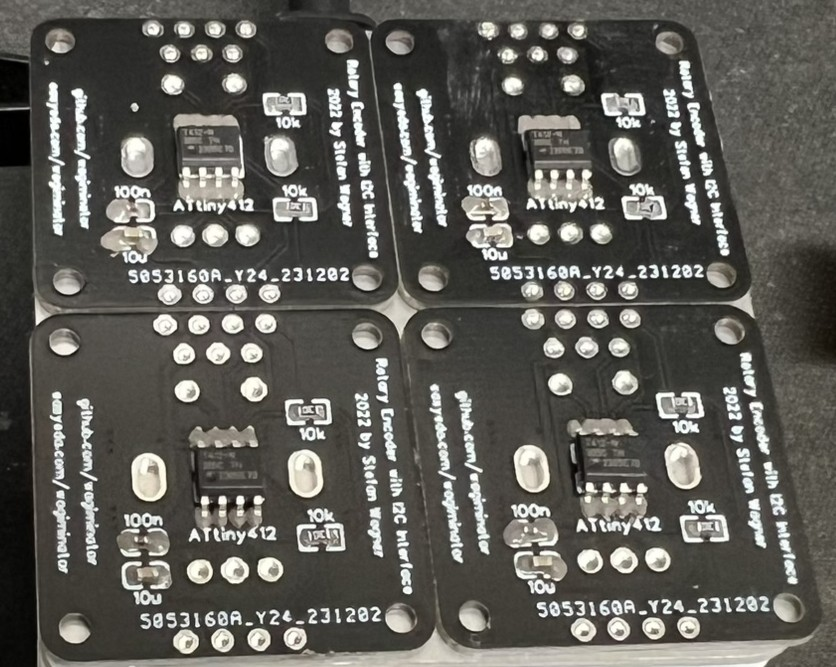
\includegraphics[scale=1]{./3_Stand_der_Technik/Abbildungen/beispiel_bild_anfertigung_reflow.JPEG}
        \caption{Symbolfoto, anfertigung von best�ckten Platinen}
    \end{minipage}
    \hfill
    \begin{minipage}[b]{0.45\textwidth}
        \centering
        \rotatebox{90}{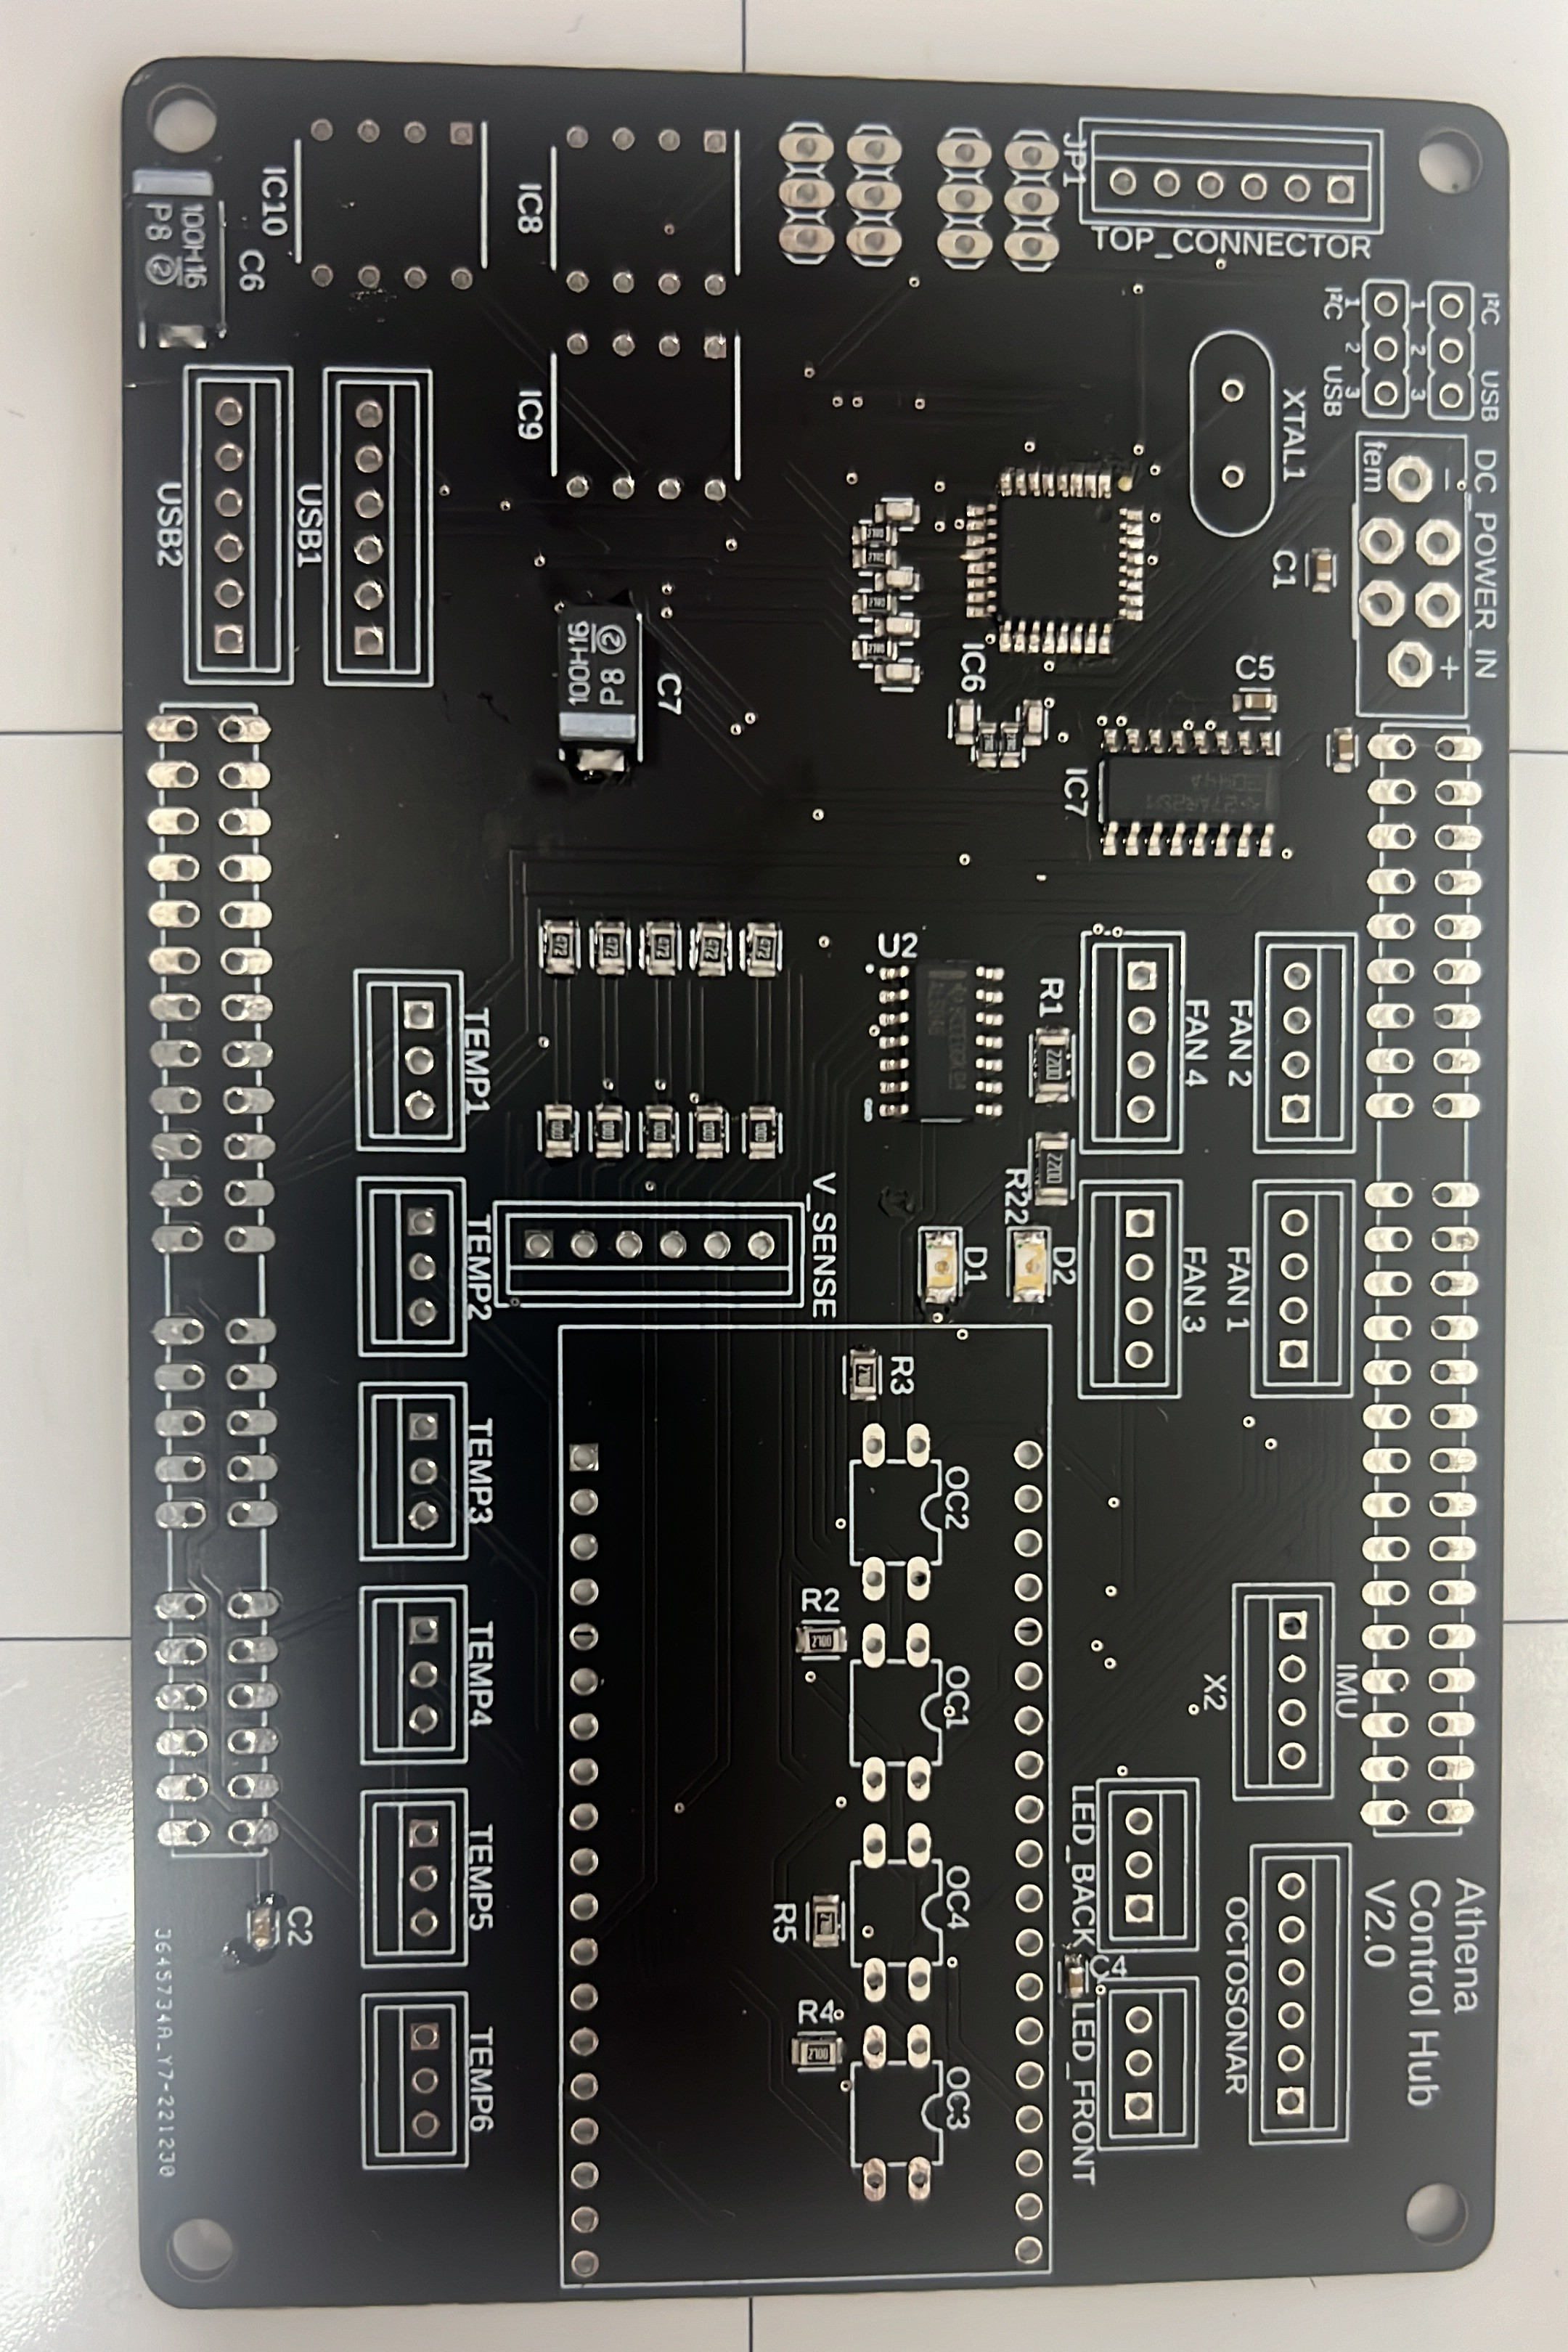
\includegraphics[scale=0.09]{./3_Stand_der_Technik/Abbildungen/shield_done.jpg}}
        \caption{Symbolfoto, fertig verl�tete Platine f�r den Bordcomputer.}
    \end{minipage}
\end{figure}


	
	\fancyfoot[C]{G�rel}
\subsection{L�ten mit L�tkolben}

Beim traditionellen L�ten mit einem L�tkolben k�nnen erfolgreich Komponenten bis zu der Gr��e 0603 (0,06 x 0,03 Zoll) verl�tet werden. Allerdings gestaltet sich das Verl�ten von SMD ICs als schwierig. Die Hitze des L�tkolbens f�hrt teilweise zu Besch�digungen der ICs und zu visuellen sowie qualitativen Unregelm��igkeiten an den L�tstellen, was die Qualit�t und Zuverl�ssigkeit der Verbindungen beeintr�chtigt. Diese Probleme verdeutlichten die Notwendigkeit einer pr�ziseren und schonenderen L�ttechnik, insbesondere f�r empfindliche Bauteile wie SMD ICs.

Es gibt grunds�tzlich zwei Unterschiede beim L�tzinn: bleihaltig und bleifrei. Bleihaltiges L�tzinn hat eine niedrigere Schmelztemperatur von etwa 190�C, was eine einfachere Handhabung erm�glicht und gute Flusseigenschaften bietet. Jedoch birgt bleihaltiges L�tzinn Gesundheitsrisiken aufgrund der Freisetzung von Bleid�mpfen w�hrend des L�tprozesses.

Im Gegensatz dazu erfordert bleifreies L�tzinn eine h�here Schmelztemperatur von etwa 220�C. Diese erh�hte Temperatur kann dazu f�hren, dass empfindliche Komponenten w�hrend des L�tprozesses leichter besch�digt werden. Dennoch bietet bleifreies L�tzinn eine sicherere Alternative f�r die Gesundheit von Mensch und Umwelt, da es keine Toxine enth�lt.

	
	\fancyfoot[C]{G�rel}
\subsection{L�ten mit Reflow-Heizplatte}

Bei dieser L�tmethode wird eine L�tpaste mithilfe einer Schablone auf die Platine aufgetragen. Die Paste besteht gr��tenteils aus Flussmittel und Tr�germaterial, die feine Zinnpartikel enthalten, die in der Fl�ssigkeit verteilt sind. Der Schmelzpunkt betr�gt 140�C und ist schonender f�r die Komponenten. Mit dieser Methode k�nnen Komponenten der Gr��e 0402 und dicht kontaktierte ICs verl�tet werden. Durch die Oberfl�chenspannung des L�tzinns werden die Komponenten bei Erhitzen zentriert auf die Pads gezogen und m�ssen nur selten leicht korrigiert werden.

Die Herstellung und der Versand der Schablone sind kostenintensiv, daher wurde das Online-Tool \textbf{\textcolor[rgb]{1,0.41,0.13}{solder-stencil.me}} genutzt. Mit diesem Tool k�nnen Schablonen f�r den 3D-Druck anhand einer Gerber-Datei erstellt werden, welche verschiedene Produktionsdateien wie das Au�enprofil, Bohrungen und Leiterbahnen enth�lt. Dieser erstellt dann eine 3D Datei mit einer festgelegten Dicke und ausschnitte �ber den L�tpads, diese k�nnen mit der Offset Korrektur relativ gesehen kleiner oder gr�sser gemacht werden um die Menge der Paste besser zu regulieren.

	
	\fancyfoot[C]{Sandri}
\section{Elektrische Antriebsmaschinen}
Elektrische Maschinen wandeln elektrische Energie in mechanische Energie um, indem sie das Prinzip der Lorenzkraft beziehungsweise Reluktanzkraft anwenden um einen Rotor zu rotieren. Der grunds�tzliche Aufbau eines elektrischen Motors besteht grunds�tzlich aus einem Stator, dem nicht-rotierendem Teil, und einem Rotor, dem sich rotierenden teil. Je nach Typ und Ausf�hrung des Motors sind auf beiden Komponenten Wicklungen beziehungweise Dauermagnete befestigt. Bei einigen Motoren sind auch noch andere Bauteile verbaut.

\subsubsection{Lorentzkraft}
	Die Lorentzkraft wirkt auf bewegliche Lasungstr�ger in einem Magnetfeld. Sie wirkt senkrecht zur Bewegungsrichtung der Ladung und senkrecht zu den Feldlinien des Magnetfelds. Wie sich die Lorentzkraft verh�lt, l�sst sich anhand folgendem Beispiel, einer Leiterschaukel erkl�ren:

	\begin{figure}[H]
			\centering
			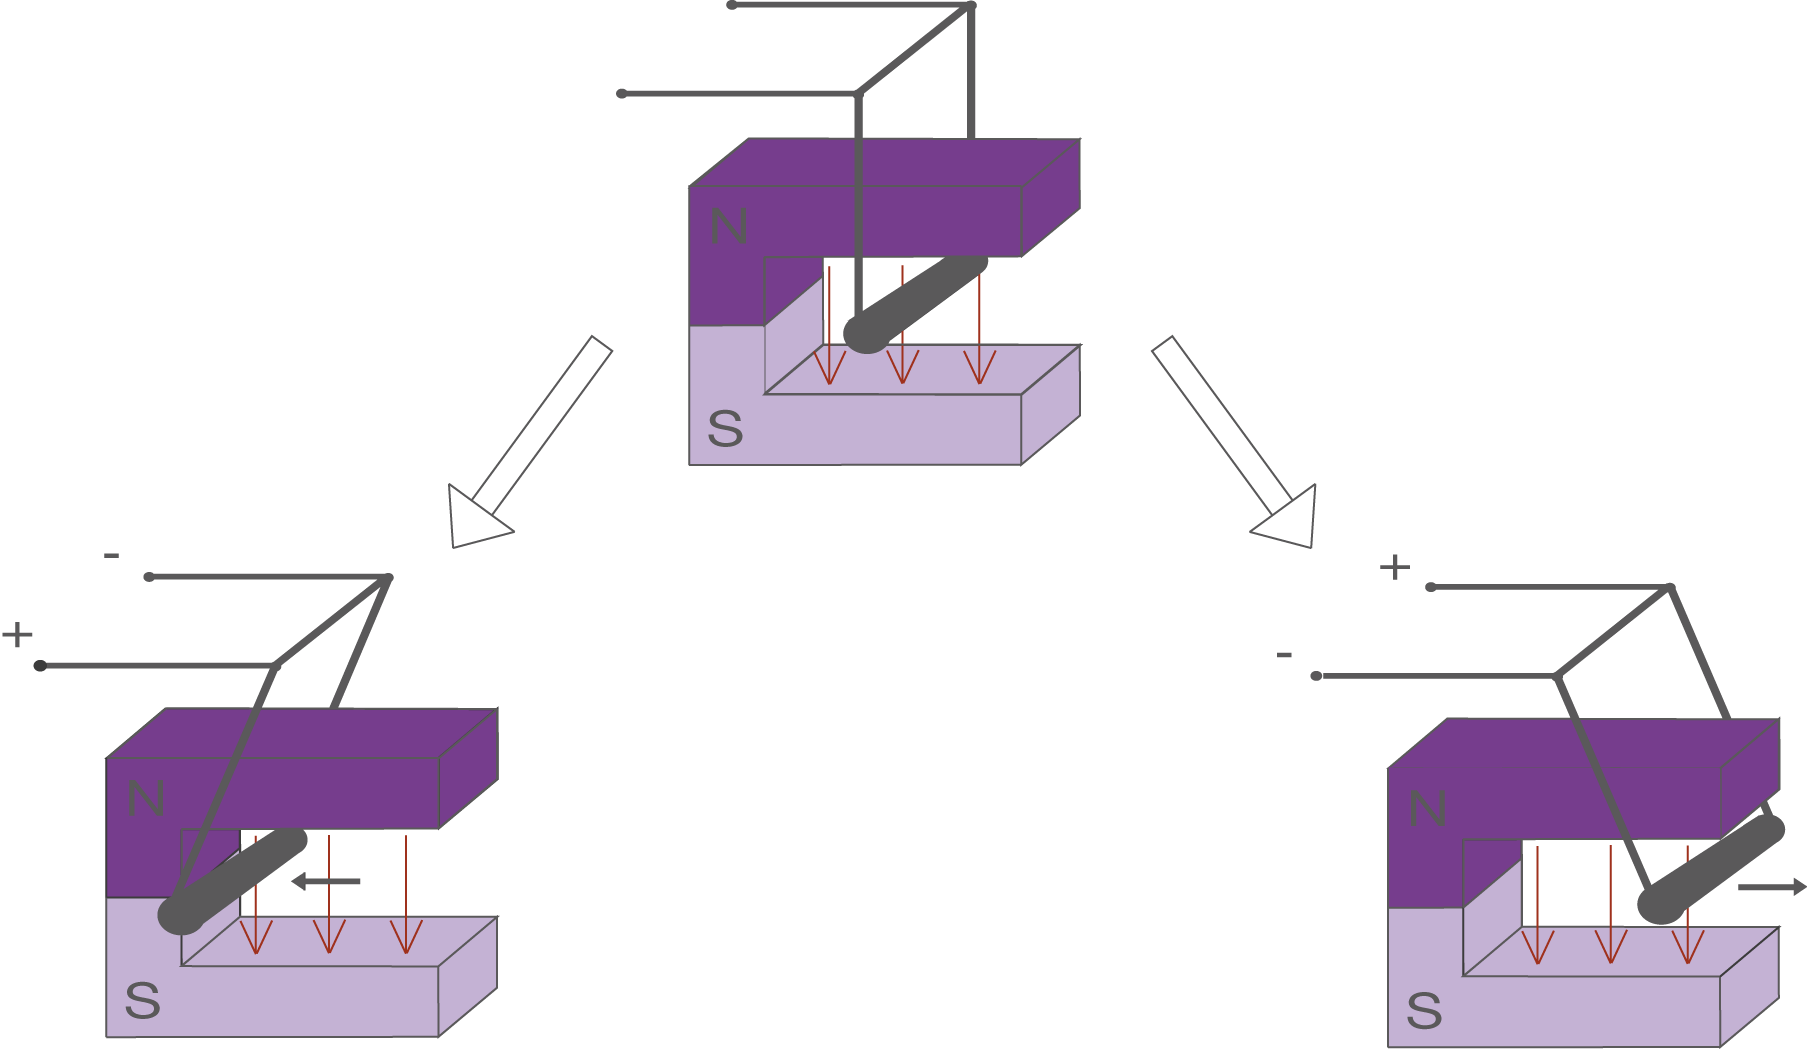
\includegraphics[scale=0.8]{./3_Stand_der_Technik/Abbildungen/Leiterschaukel_1}
			\caption{�nderung der Stromrichtung Lorentzkraft\cite{schullv.de2024}}
	\end{figure}
	
	Die Richtung in welche die Leiterschaukel ausschl�gt, ist zum einen Abh�ngig von der Richtung des Stroms und zum anderen von der Orientierung des Magnetfelds.
	
	\begin{figure}[H]
			\centering
			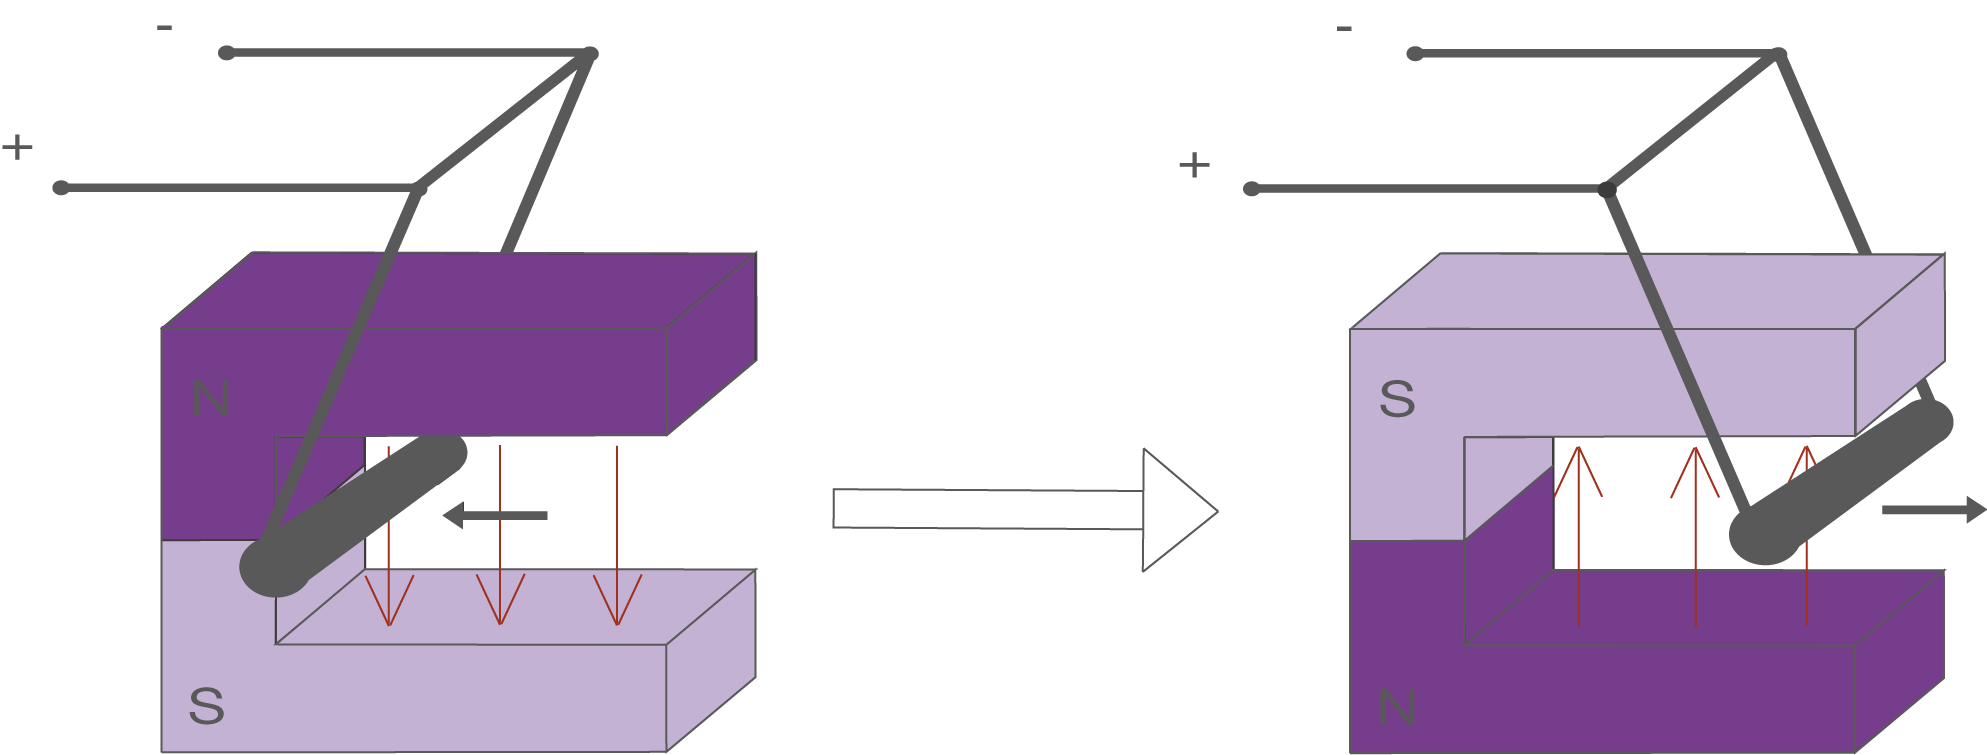
\includegraphics[scale=0.8]{./3_Stand_der_Technik/Abbildungen/Leiterschaukel_2}
			\caption{�nderung des Magnetfelds Lorentzkraft\cite{schullv.de2024}}
	\end{figure}
	
	Die Richtung der Lorentzkraft kann auch durch einen einfachen Versuch, den linke Hand Versuch, ermittelt werden:
	
	\begin{figure}[H]
			\centering
			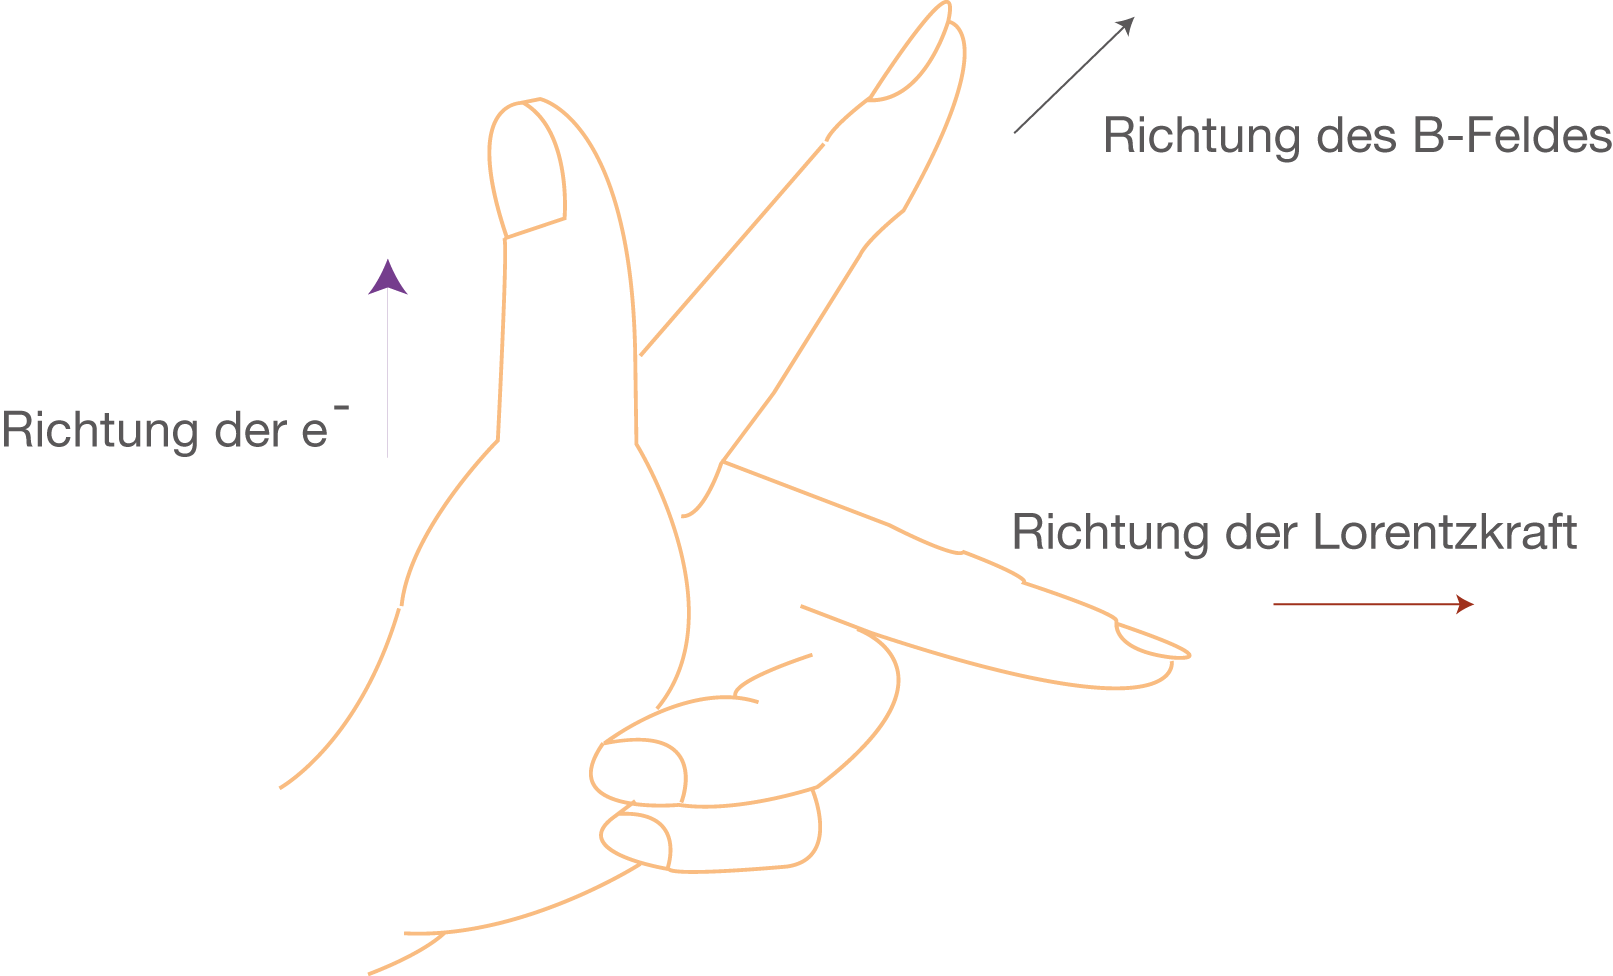
\includegraphics[scale=0.8]{./3_Stand_der_Technik/Abbildungen/Lorentzkraft_1}
			\caption{Die linke Hand Regel\cite{schullv.de2024}}
	\end{figure}

	Mathematisch kann die Richtung der Lorentzkraft mihilfe des Kreuzprodukts aus der Magnetfeldrichtung und der Bewegungsrichtung der Elektronen errechnet werden:
	
	\begin{equation}
		\vec{F_{L}} = q * (\vec{v_{e}} \times \vec{B})
	\end{equation}
	
	Der Betrag kann wiefolgt errechnet werden:
	
	\begin{equation}
		F_{L} = q*v*B*\sin{\alpha}
	\end{equation}
	
	Wobei der Winkel $\alpha$ den Winkel zwischen der Bewegungsrichtung der Elektronen und der Bewegungsrichtung des Magnetfelds entspricht. Auch kann man anhand dieser Formel erkennen, dass die Lorentzkraft null wird, wenn die Bewegungsrichtung der Elektronen und die des Magnetfelds parallel verl�uft.\cite{schullv.de2024}
	
	Die meisten elektrischen Maschinen funktionieren grunds�tzlich aufgrund der Lorentzraft, es gibt jedoch vereinzelt Maschinen, die nur aufgrund der Reluktanzkraft funktionieren.

\subsubsection{Reluktanzkraft}

	Die Reluktanzkraft (auch Maxwellsche Kraft genannt) entsteht durch �nderung des magnetischen Widerstands. Sie wirkt immer so, dass sich der magnetische Widerstand verringert und die Induktivit�t steigt. Diese Kraft kann durch Ver�nderung des Luftspalts im magnetischen Kreis erzeugt werden.\cite{biancahoegel.de/2021}
	
	\subsection{Asynchronmaschine}
	Die Asynchronmaschine ist die einfachste Form einer elektrischen Maschine. Sie wird angetrieben durch ein Drehfeld, welches durch eine mehrstr�ngige Wicklung im Stator erzeugt wird. Der gro�e Vorteil des Asynchronmaschine ist ihre einfache Bauform und Funktionsweise. Auch bedarf sie nur geringer Wartung. Der gro�e Nachteil hingegen ist jedoch seine startk an die Frequenz der Eingangsspannung gebundene Drehzahl. Im gebr�uchlichen 50-Hz-Betrieb sind nur Drehzahlen von 3000U/min, 1500U/min, 1000U/min, abh�ngig von der Anzahl der Polpaare.
	
	\begin{equation}
		n \thickapprox f / p
	\end{equation}
	
	n $\cdots$ Motordrehzahl \newline
	f $\cdots$ Frequenz vom Netz	\newline
	p $\cdots$ Anzahl der Polpaare \newline
	
	Es gibt haupts�chlich zwei Typen der Asynchronmaschine, den K�figl�ufer und den Schleifringl�ufer. Der K�figl�ufer verwendet also Rotor eines Stahlk�fig, der Schleifringl�ufer hat Schleifringe, �ber die Wicklungen im Rotor bestromt werden.
	
	\begin{figure}[H]
			\centering
			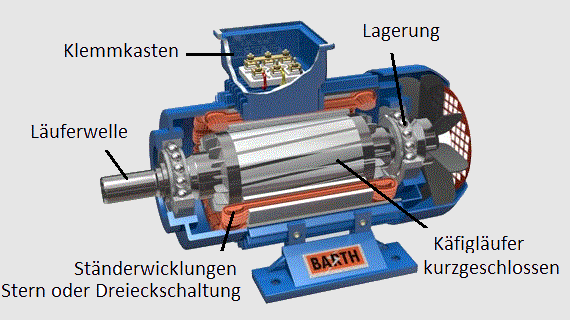
\includegraphics[scale=0.6]{./3_Stand_der_Technik/Abbildungen/Asynchronmaschine_2}
			\caption{Aufbau K�figl�ufer\cite{kfzaufgaben.de2024}}
	\end{figure}
	
	\begin{figure}[H]
			\centering
			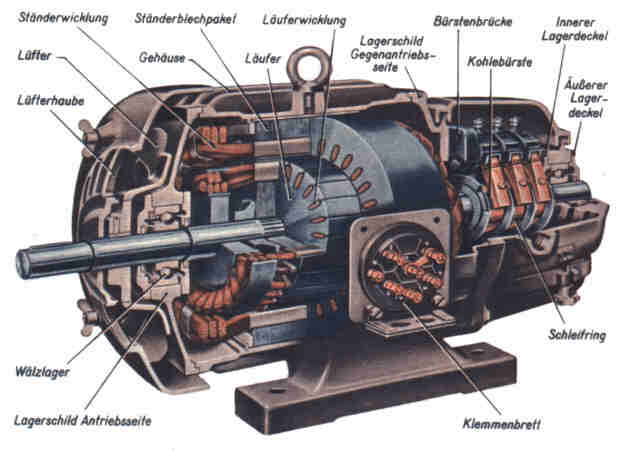
\includegraphics[scale=2]{./3_Stand_der_Technik/Abbildungen/Asynchronmaschine_3}
			\caption{Aufbau Schleifringl�ufer\cite{wupperindustrie.de2024}}
	\end{figure}

	Betrieben wird die Asynchronmaschine indem sie an das 3-phasige 50Hz-Netz angeschlossen wird. Sie dreht sich dadurch fast synchron mit der Netzfrequenz. Asynchronmaschinen laufen ihrem Feld jedoch immer etwas hinterher, diese Eigenschaft nennt man Schlupf. Das Drehmoment- und Drehzahlverhalten kann sehr gut mittels eines Kreisdiagramms dargestellt werden.\cite{Fischer2017}
	
	\begin{figure}[H]
			\centering
			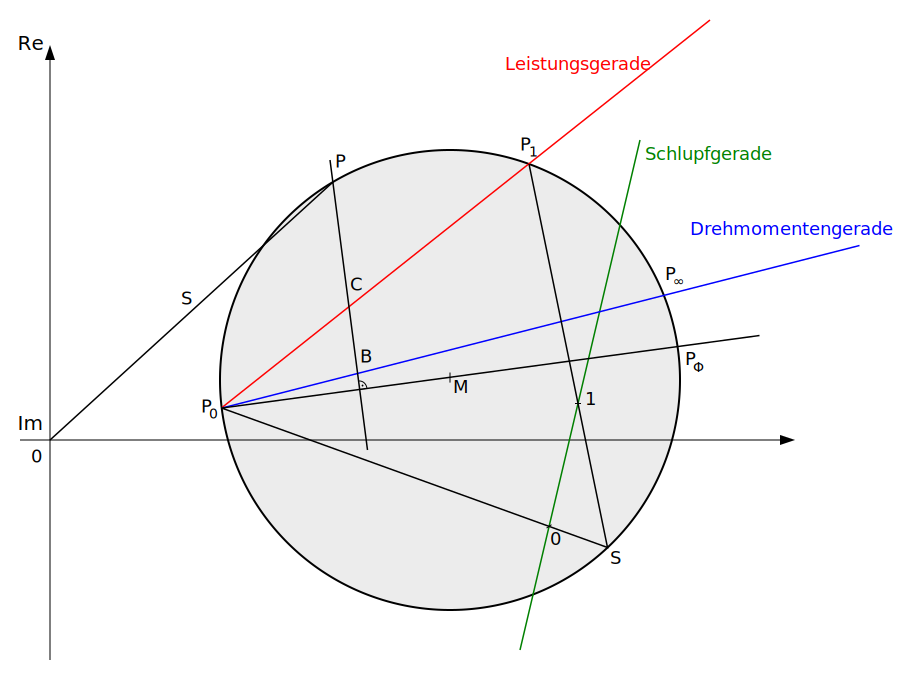
\includegraphics[scale=0.4]{./3_Stand_der_Technik/Abbildungen/Kreisdiagramm_1}
			\caption{Kreisdiagram eines Asynchronmotors\cite{Wikipedia2024}}
	\end{figure}
	
	
	
	\subsection{Gleichstrommaschine}
	
	\subsection{Synchronmaschine}
	
	\subsection{Positionsmessung}
	Um Motoren genau Regeln zu k�nnen ist es meistens n�tig die Position des Rototrs zu messen. Dies kann wie folgt umgesetzt werden:

	\subsubsection{Back-EMF}
		Wenn in einer Spule sich der Stromfluss �ndert, wird eine Spannung induziert, im Fall von Synchronmaschinen wird diese Spannung Back-EMF genannt. Diese kann gemessen werden und es kann anhand dieser die Position und Drehzahl des Rotors ermittelt werden.
		
	\begin{figure}[H]
			\centering
			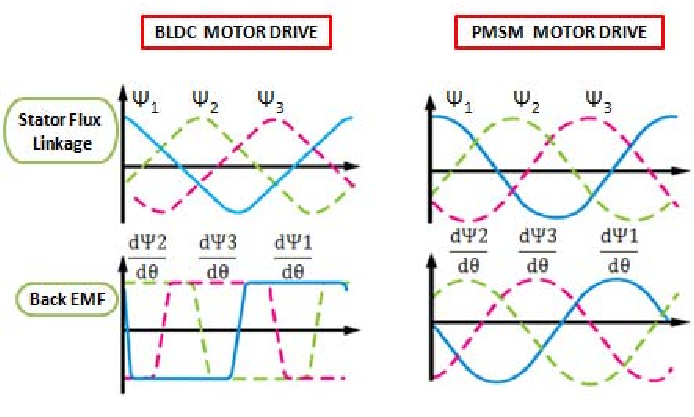
\includegraphics[scale=0.5]{./3_Stand_der_Technik/Abbildungen/PMSM_Back-EMF_1}
			\caption{Back-EMF Synchronmaschine\cite{Rode2023}}
	\end{figure}
	
	\subsubsection{Hall-Sensoren}
		Hall-Sensoren k�nnen sind Halb
	
	\subsubsection{Resolver}
	
	\subsection{BLDC Regelung}\label{Trapezfoermige Regelung}
%%BLDC Motor wird auch Blockstrommotor genannt
	BLDC-Motoren werden meistens mit einem einfachen Regler bestehend aus 6 MOSFETs geregelt. Mithilfe von diesen kann jede Phase des Motors auf entweder VCC(Versorgungsspannung) oder GND(Nullpotenzial) geschalten werden. 
	
	\begin{figure}[H]
			\centering
			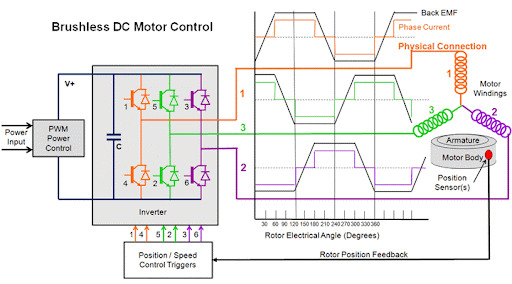
\includegraphics[scale=0.7]{./3_Stand_der_Technik/Abbildungen/BLDC_Control_3}
			\caption{BLDC-Regler\cite{settech.com.tw2024}}
	\end{figure}
	
	\begin{figure}[H]
			\centering
			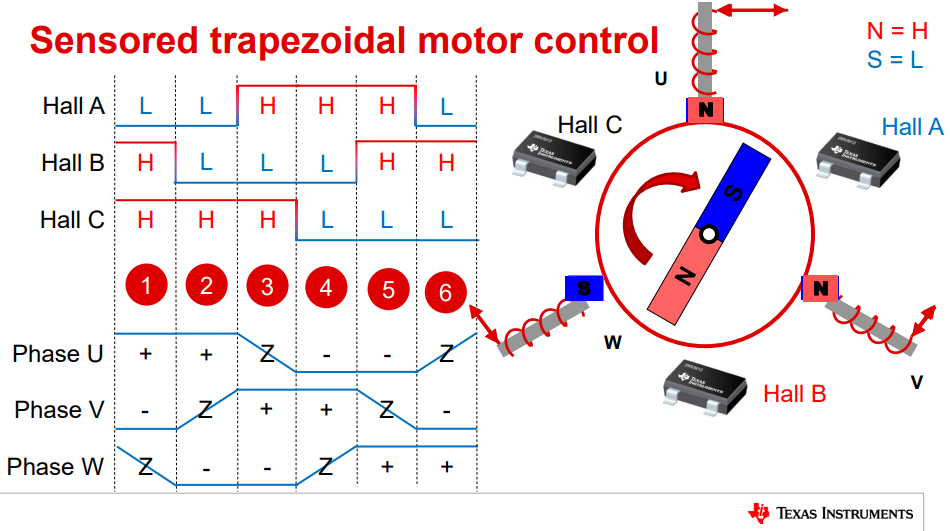
\includegraphics[scale=0.5]{./3_Stand_der_Technik/Abbildungen/BLDC_Control_4}
			\caption{Eine Rotation\cite{settech.com.tw2024}}
	\end{figure}
	
	Zus�tzlich zu den 6 MOSFETs besteht die Schaltung aus einigen Komponenten zur Spannungsstabilisierung und aus einer Kontrolleinheit. Diese Kontrolleinheit misst die Rotoposition(siehe \ref{Positionsmessung}) und schaltet die MOSFETs dementsprechend. Dadurch entsteht ein sechs-stufiger Ablauf. Die Anzahl an Positionen, die ein Motor mithilfe dieser Regelmethode annehemen kann, ergibt sich aus dem sechsfachen der Polpaare des Motors. Im Optimalfall sollte das Rotorfeld dem Statorfeld um 90� vorlaufen um maximales Drehmoment zu erzeugen. Bei dieser Regelung variiert es jedoch immmer zwischen 60� und 120�, was dazu f�hrt, dass das Drehmoment im Laufe einer Rotation merhmals zu- und abnimmt. Auch die Geschwindigkeit ist w�hrend einer Umdrehung nicht ganz konstant.
	
	\begin{figure}[H]
			\centering
			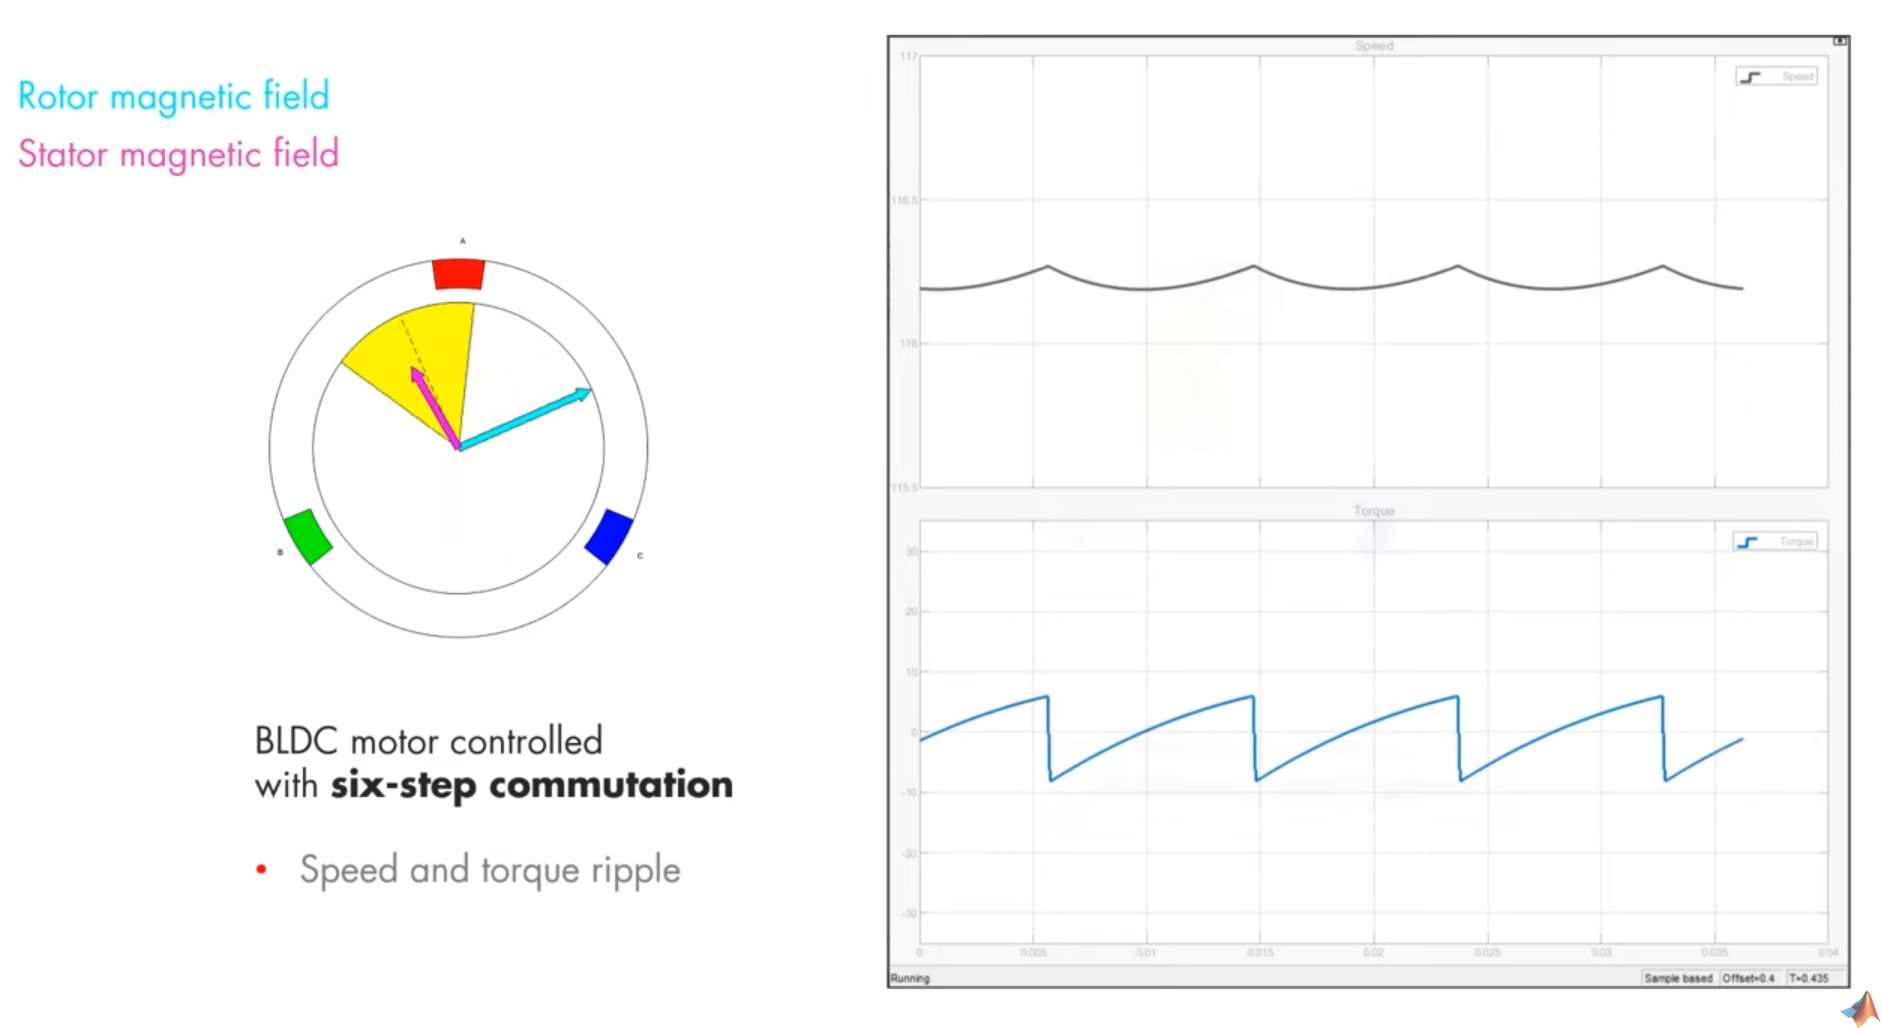
\includegraphics[scale=0.3]{./3_Stand_der_Technik/Abbildungen/BLDC_Control_1}
			\caption{Feld und Drehmoment bei BLDC-Regelung\cite{MATLAB2020}}
	\end{figure}
	
	\subsection{Feldorientierte Regelung (FOC)}\label{Feldorientierte Regelung}
	Mithilfe der feldorientiereten Regelung ist es m�glich das Feld des Stators so anzupassen, dass es dem Feld des Rotors genau so vorl�uft, dass Drehmoment und Effizienz maximiert werden. Im Gegensatz zur BLDC-Regelung kann das Statorfeld nicht nur 6 Positionen annehmen, sondern unbegrenzt viele. Man kann mit dieser Methode auch eine etwas h�here Drehzahl erreichen. Um diese 90� Verschiebung des Statorfelds zu erreichen, wird der Feldvektor zun�chst in seine zwei Komponenten Id und Iq aufgeteilt:
	
	\begin{figure}[H]
			\centering
			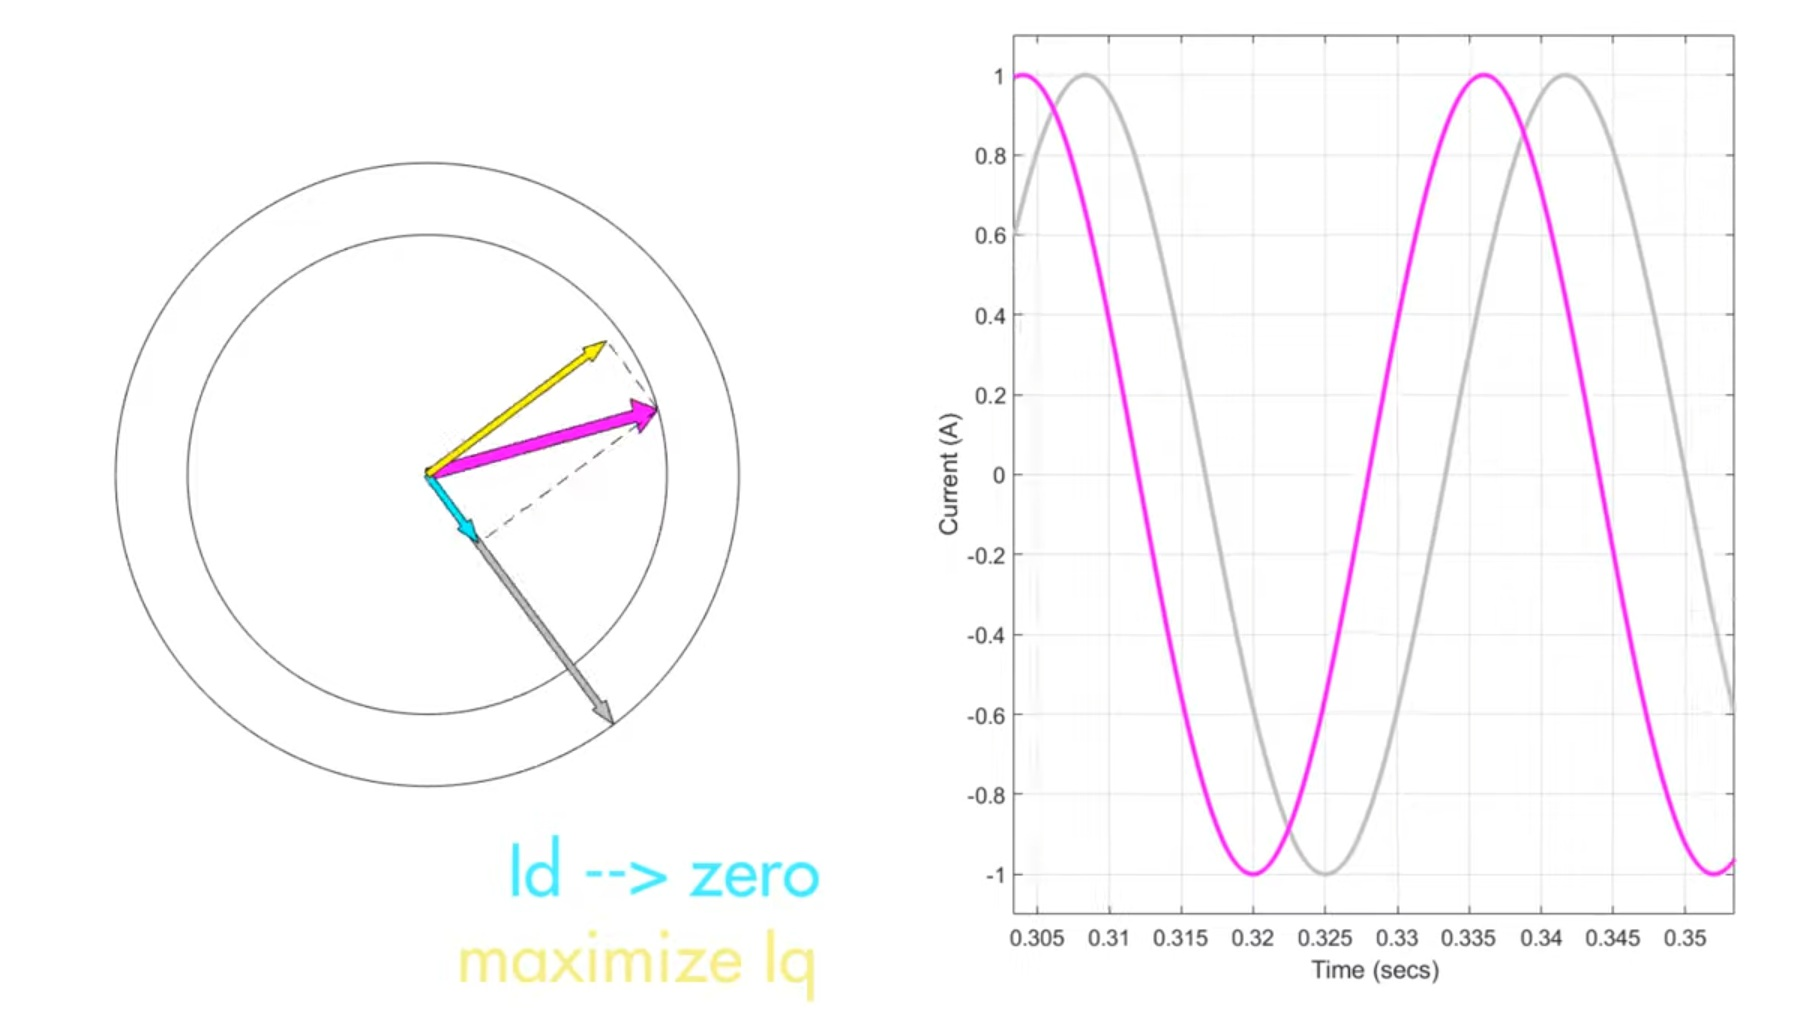
\includegraphics[scale=0.3]{./3_Stand_der_Technik/Abbildungen/FOC_Control_1}
			\caption{Komponenten des Statormagnetfelds\cite{MATLAB2020}}
	\end{figure}
	
	Das Ziel des Reglers ist demnach Id gegen 0 zu regeln und Iq entsprechend dem gew�nschten Drehmoment so hoch wie m�glich zu regeln.
	
	Der Aufbau eines FOC-Algorhitmus ist in der Regel wiefolgt:
	
	\begin{figure}[H]
			\centering
			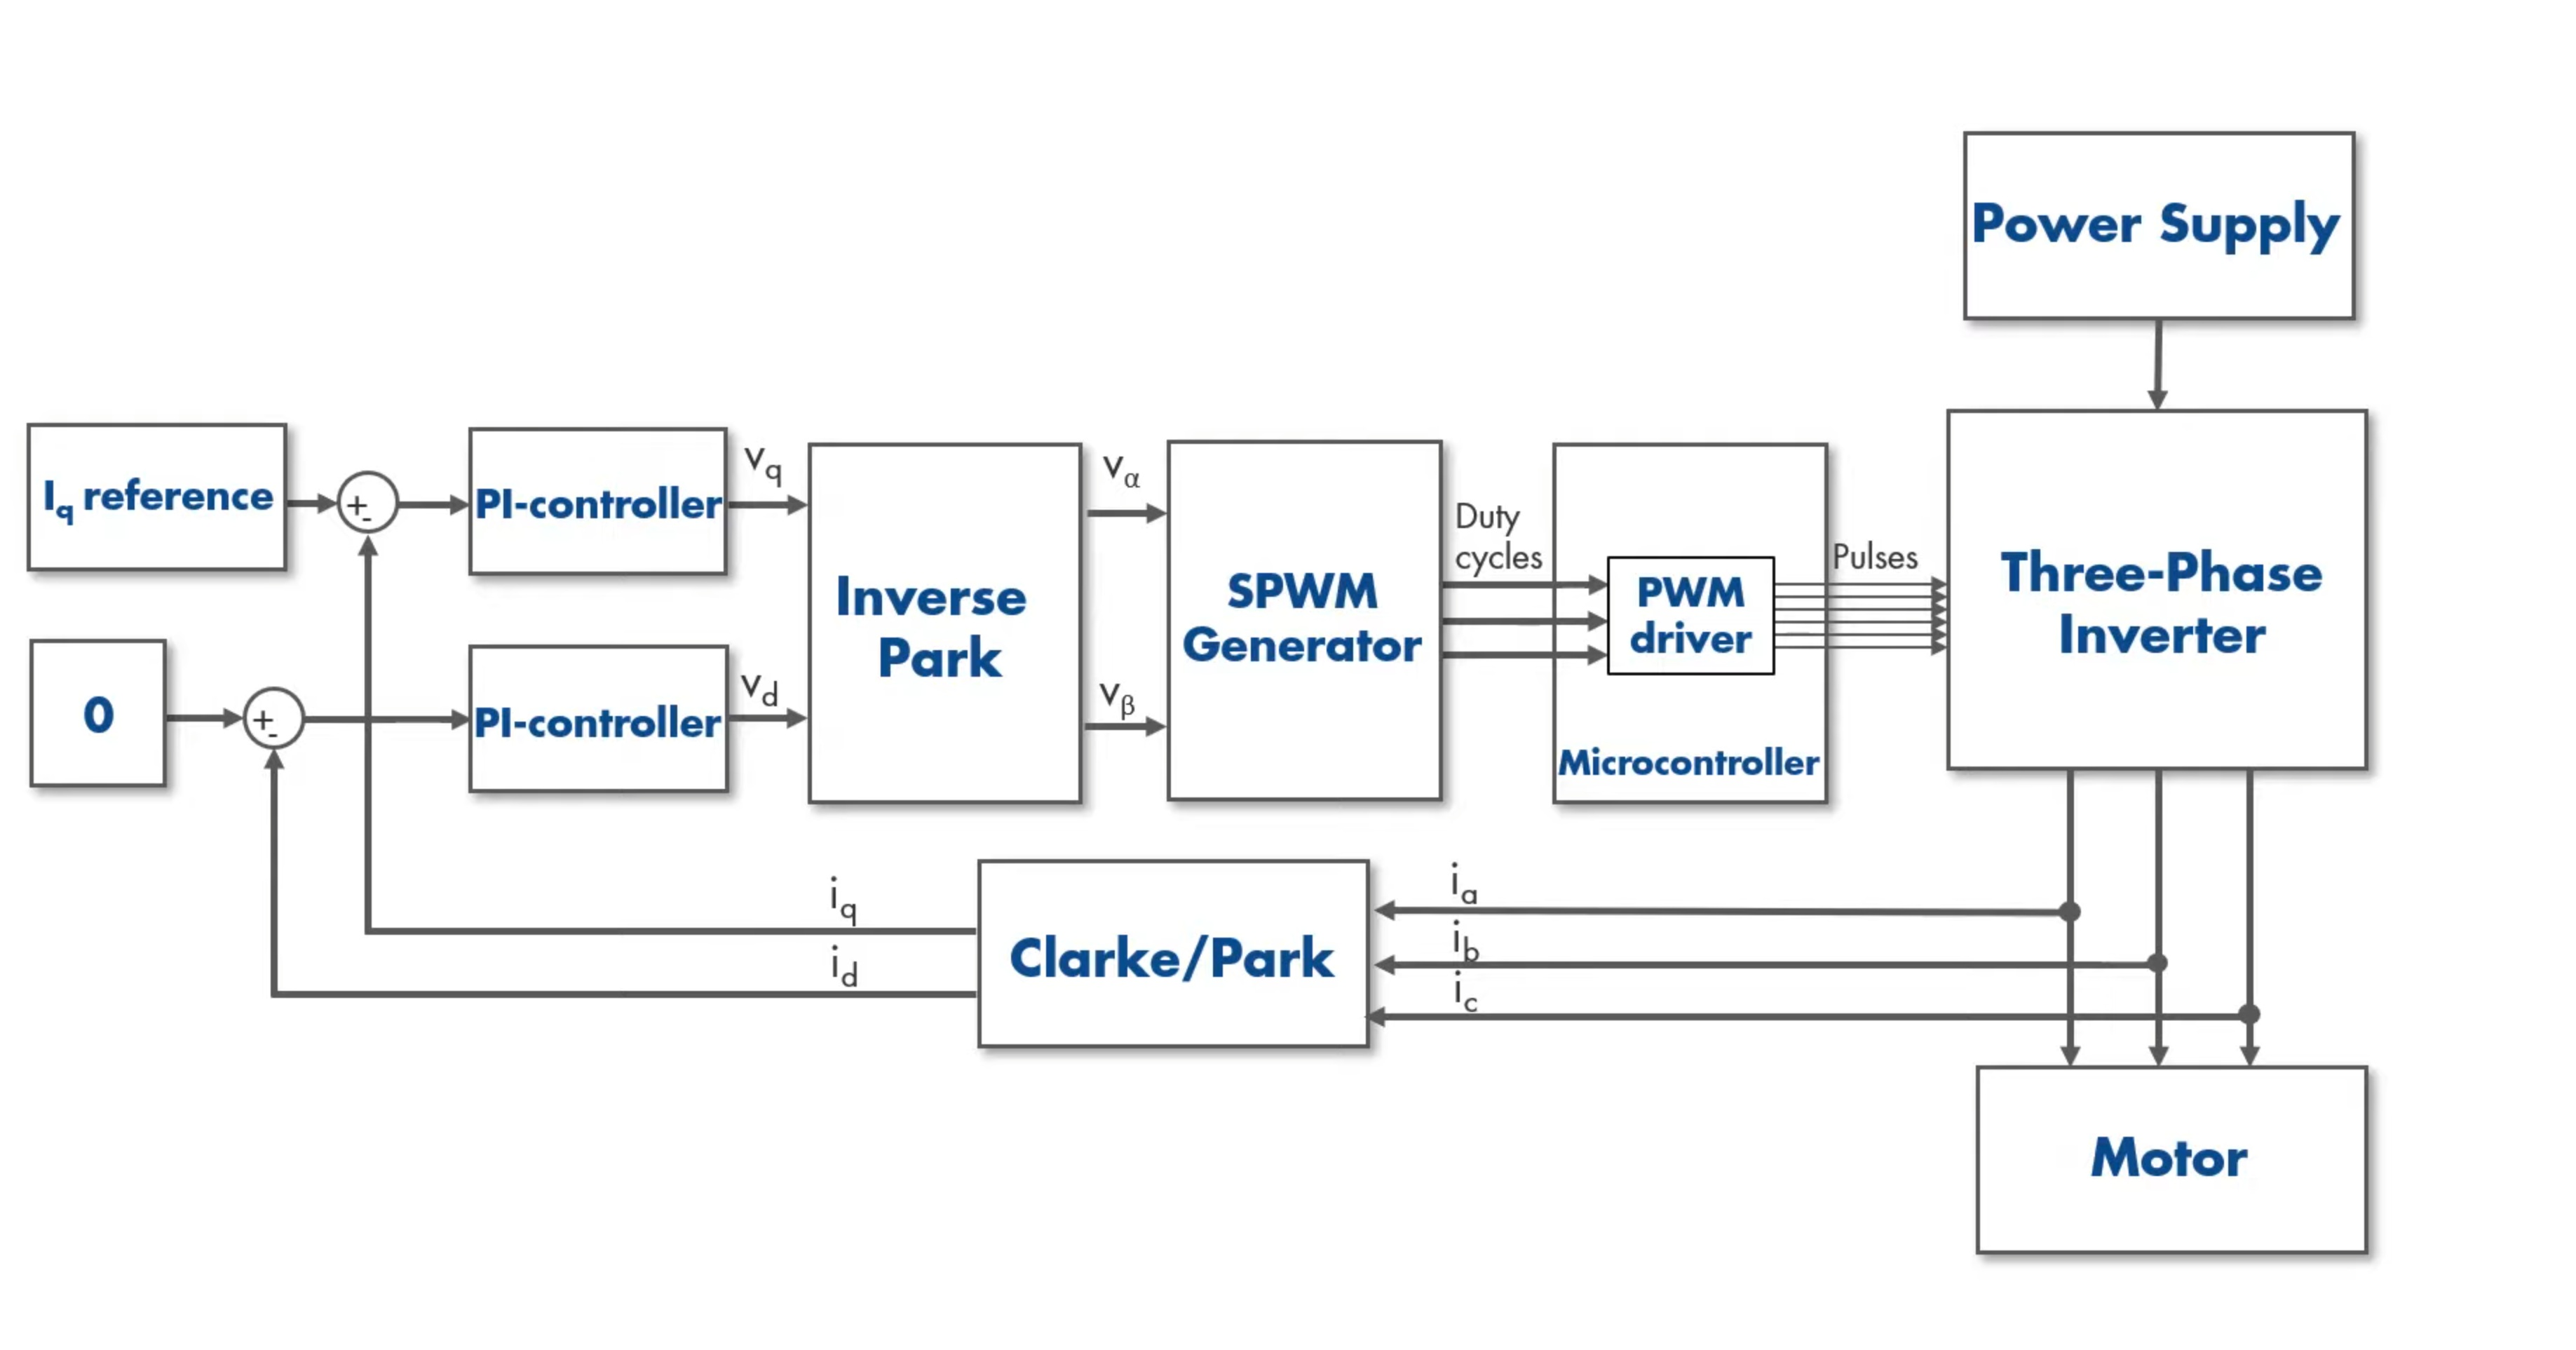
\includegraphics[scale=0.3]{./3_Stand_der_Technik/Abbildungen/FOC_Control_2}
			\caption{Aufbau eines FOC-Algorhitmus\cite{MATLAB2021}}
	\end{figure}
	
	Mithilfe von Shunts wird der derzeitige Strom zum Motor gemessen. Diese Werte werden mithilfe von mathematischen Transformationen (Clark- und Park Transformation) in die zwei Anteile Id und Iq aufgeteilt. Auch wird mithilfe eines Positionssensors die Position des Rotors gemessen.
	Zwei PI-Regler regeln nun Id auf 0 und Iq auf den gew�nschten Strom. Anschlie�end werden die Werte mithilfe von mathematischen Transformationen(inverse Clark Transformation) in die gew�nschten Spannungswerte Vd und Vq umgerechnet. 
	
	\section{Spannungsversorgung}
	Test
	
	\section{Sensorik}
	\subsection{LiDAR Sensoren}
LiDAR-Sensoren sind ein essenzielles Instrument in der modernen Sensorik, welche erm�glichen, pr�zise Messungen der Umgebungen zu erstellen. 
Die einfachsten Sensoren bestehen aus einem Time-of-Flight (TOF) Distanzmesser, welches einen Lichtpuls sendet und die Zeit misst, die es f�r die R�ckkehr ben�tigt. 
Die LiDAR Sensoren werden grunds�tzlich in 3 Kategorien aufgeteilt:

\textbf{1D-LiDAR}
In seiner grundlegendsten Form besteht der LiDAR-Sensor aus einem Distanzmesser, der seine Reichweite in einer einzigen Dimension misst. 
Dieser Ansatz erm�glicht eine schnelle Erfassung von Entfernungen entlang einer Linie, was als 1D-LiDAR bekannt ist. 
Die Genauigkeit dieser Messungen h�ngt von verschiedenen Faktoren ab, wie der Leistung des Laserimpulses, der Empfindlichkeit des Photosensors und der Rotationsgeschwindigkeit der Basis. 
Diese Ger�te sind im Handwerk verbreitet und haben bei geringen Kosten eine hohe Genauigkeit.

\textbf{2D-LiDAR}
Durch die kontinuierliche Rotation des Distanzmessers um eine Achse wird der 1D-LiDAR zu einem 2D-LiDAR erweitert. 
Diese Erweiterung erm�glicht eine Erfassung von Entfernungen entlang einer Linie und gleichzeitig um die eigene Achse herum. 
Dadurch entsteht eine 2D-Karte der Umgebung, die eine detailliertere Darstellung erm�glicht. 
Diese Ger�te sind mechanisch komplex, da der Sensor im Idealen Fall bei exakt gleich bleibender Geschwindigkeit genau horizontal gedreht werden muss. 
Diese Sensoren sind bei autonomen Ger�ten im Indoor-Bereich verbreitet, wie zum Beispiel ein Saug-Roboter oder ein autonomes Lieferfahrzeug in einer Lagerhalle.

\begin{figure}[H]
    \centering
    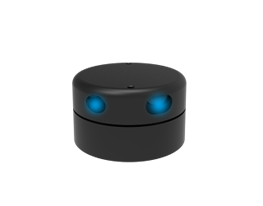
\includegraphics[scale=0.55]{./3_Stand_der_Technik/Abbildungen/symbolfoto_lidar_C_YDLIDAR.png}
    \caption{Symbolfoto 2D LiDAR Sensor, YDLiDAR G2 \cite{YDLiDAR2024}}
\end{figure}

\textbf{3D-LiDAR}
Ein weiterer Fortschritt in der LiDAR-Technologie ist der 3D-LiDAR, der nicht nur um eine Achse rotiert, sondern auch in der H�he verstellbar ist. Durch diese zus�tzliche Dimension werden bestimmte H�hen nacheinander abgetastet, wodurch eine vollst�ndige dreidimensionale Punktwolke der Umgebung erstellt wird. Diese Ger�te haben entweder mehrere gestapelte Sensoren um eine Art Punktwolke zu erstellen oder modifizieren die H�he des Lasers von einer einzelnen Quelle. Die Genauigkeit und Aufl�sung dieser Punktwolke h�ngt von der Art des Sensors sowie die Pr�zision und der Rotationsmechanik ab.

\textbf{Anwendung und Bedeutung}
LiDAR-Sensoren finden in verschiedenen Anwendungen Anwendung, darunter Gel�nde- und Geb�udevermessung sowie Unterst�tzung autonomer Fahrzeuge. Die M�glichkeit, pr�zise Entfernungen zu messen und detaillierte 3D-Karten zu erstellen, macht sie unverzichtbar f�r Projekte, die eine genaue Umgebungswahrnehmung erfordern. Die Erfassung der Intensit�t des reflektierten Lichts erm�glicht zudem eine detaillierte Oberfl�chencharakterisierung, was in vielen Anwendungen von gro�em Nutzen ist.

	
	\subsection{Ultraschallsensoren}
Ultraschallsensoren bestehen aus einem Schallwandler und einer Empfangseinheit. Der Schallwandler sendet Ultraschallwellen aus, die an Objekten reflektiert werden und von der Empfangseinheit erfasst werden. 
Tonwellen ab 20 kHz gelten als Ultraschall und k�nnen demnach nicht vom Menschen geh�rt werden, die Sensoren operieren unter diesem Bereich \cite{Frantzen2024}. 
Die Zeitmessung zwischen Aussenden und Empfangen des Schallsignals erm�glicht die Berechnung der Entfernung zum Objekt. 

Ultraschallsensoren bieten eine kosteng�nstige L�sung f�r die Abstandsmessung und werden h�ufig als Fahrzeugparkassistenz oder in der Robotik verwendet. Der generelle Anwendungsbereich ist jener, bei dem eine grobe Ann�herung der Entfernung ausreicht.

		
	\fancyfoot[C]{G�rel}
\subsection{Radar Sensoren}
Radar (Radio Detection and Ranging) Sensoren bestehen aus einer Sendeantenne und einer Empfangsantenne. Die Sendeantenne sendet hochfrequente elektromagnetische Wellen aus, die von Objekten reflektiert werden und von der Empfangsantenne erfasst werden. Die Zeitmessung zwischen Aussenden und Empfangen des Signals erm�glicht die Berechnung der Entfernung zum Objekt. 

Radar bietet eine effektive M�glichkeit, Entfernungen zu messen und Bewegungen zu verfolgen. Es wird h�ufig in der Luft- und Seefahrt, der Wetterbeobachtung, der Verkehrs�berwachung und der milit�rischen Anwendung eingesetzt. Im Vergleich zu LiDAR und Ultraschallsensoren bietet Radar eine gr��ere Reichweite und ist weniger anf�llig f�r Umwelteinfl�sse wie Nebel oder Regen.

	
	\subsection{Kameras}
Kameras haben eine entscheidende Rolle in der Personenerkennung und im Bereich der K�nstlichen Intelligenz (KI), insbesondere in Anwendungen wie Video�berwachung, Gesichtserkennung und biometrischer Authentifizierung. Verschiedene Aspekte der Kamera, wie Objektiv, Fokus und Blende, beeinflussen die Leistung und Genauigkeit dieser Anwendungen.

\textbf{Objektiv:} Das Objektiv einer Kamera bestimmt, wie Licht auf den Bildsensor f�llt und beeinflusst somit die Bildqualit�t und Sch�rfe. In Anwendungen der Personenerkennung ist ein hochwertiges Objektiv wichtig, um klare und detaillierte Bilder aufzunehmen. Die Wahl des Objektivs h�ngt von den spezifischen Anforderungen der Anwendung ab, wie zum Beispiel dem Blickwinkel und der Entfernung zum zu erfassenden Objekt.

\textbf{Fokus:} Der Fokus einer Kamera bestimmt, welche Teile eines Bildes scharfgestellt werden und welche unscharf bleiben. In der Personenerkennung ist ein breiter Fokusbereich von entscheidender Bedeutung, um Personen klar und deutlich zu erfassen, unabh�ngig von ihrer Entfernung zur Kamera. Ausserdem kann ein schneller Autofokus es der Kamera erm�glichen, sich schnell an sich bewegende Personen anzupassen und klare Bilder aufzunehmen.

\textbf{Blende:} Die Blende einer Kamera reguliert die Menge an Licht, die auf den Bildsensor f�llt, und beeinflusst somit die Belichtung und Tiefensch�rfe eines Bildes. In Anwendungen der Personenerkennung ist eine angemessene Belichtung entscheidend, um klare und gut sichtbare Bilder zu gew�hrleisten, insbesondere bei unterschiedlichen Lichtverh�ltnissen. Eine variable Blende kann dabei helfen, sich an wechselnde Lichtbedingungen anzupassen und optimale Ergebnisse zu erzielen.

\textbf{Anwendung im KI-Bereich:} Im Bereich der K�nstlichen Intelligenz werden Kameras h�ufig f�r die Erfassung von Trainingsdaten verwendet, um KI-Modelle f�r die Personenerkennung zu trainieren. Hochaufl�sende Bilder, die von Kameras aufgenommen werden, dienen als Eingabe f�r diese Modelle, um Personen zu identifizieren und zu klassifizieren. Die Qualit�t der aufgenommenen Bilder, die durch die oben genannten Faktoren beeinflusst wird, tr�gt wesentlich zur Leistungsf�higkeit und Genauigkeit der KI-Modelle bei.

	
	
	\section{Rechensysteme}
	Test
	
	\section{Softwareentwicklung}
	Test

%% Mechanik %%%%%%%%%%%%%%%%%%%%%%%%%%%%%%%%%%%%%%%%%%%%%%%%%
\newpage
\chapter{Mechanik}
	TEST

%% Elektronik %%%%%%%%%%%%%%%%%%%%%%%%%%%%%%%%%%%%%%%%%%%%%%%
\newpage
\chapter{Elektronik}
	TEST

%% Software %%%%%%%%%%%%%%%%%%%%%%%%%%%%%%%%%%%%%%%%%%%%%%%%%
\newpage
\chapter{Software}
	
	\fancyfoot[C]{Sandri}
\section{Programmierung des ESP32-Mikrocontrollers}
	Die Aufgaben des ESP32 bestehen aus dem Auslesen aller Sensordaten, dem Steuern der Beleuchtung und der Kommunikation mit dem Bordcomputer. Da der ESP32 2 Kerne besitzt wird der Code zwischen diesen aufgeteilt, das Einlesen aller Sensoren und die Kommunikation l�uft auf Kern 0, das Programm f�r die Beleuchtung auf Kern 1. Um den beiden Kernen getrennt Aufgaben zuordnen zu k�nnen, m�ssen im void Setup() 2 Tasks, welche an einen bestimmten Kern gebunden sind, erstellt werden.
	
	\lstset{style=VS2017}
	\begin{lstlisting}[language=C, caption={ESP32 2 Kerne Setup}]
void setup() {

	Serial.begin(115200);

	xTaskCreatePinnedToCore(
				Task1setup,   /* Task function. */
				"Task1",     /* name of task. */
				10000,       /* Stack size of task */
				NULL,        /* parameter of the task */
				1,           /* priority of the task */
				&Task1,      /* Task handle to keep track of created task */
				0);          /* pin task to core 0 */                  
	delay(500); 

	xTaskCreatePinnedToCore(
				Task2setup,   /* Task function. */
				"Task2",     /* name of task. */
				10000,       /* Stack size of task */
				NULL,        /* parameter of the task */
				1,           /* priority of the task */
				&Task2,      /* Task handle to keep track of created task */
				1);          /* pin task to core 1 */
	delay(500);

}
	\end{lstlisting}
	

	\subsection{Kern 0 / Sensoren und Kommunikation}
	Die Hauptaufgabe von Kern 0 ist es, mit dem Bordcomputer zu kommuniziern, alle Sensordaten auszulesen, und Komponenten, wie zum Beispiel L�fter, zu steuern.
	Die Seriellen Schnittstellen vom ESP32 und dem Bordcomputer sind mithilfe des Shields verbunden, um eine fl�ssige Kommunikation zu gew�hrleisten, ist ein Protokoll n�tig:
	
	\subsubsection{Aufbau von Paketen zwischen ESP32 und Bordcomputer}
		Der grunds�tzliche Aufbau eines Paktes zwischen ESP32 und Bordcomputer ist immer gleich, er besteht aus folgenden Teilen
			
			\begin{enumerate}
			
				\item Datentyp: LED, Temp, Volt, IMU1, IMU2, Sonar, FAN, Error //Alle m�glichen Daten, die zwischen ESP und Bordcomputer gesendet werden k�nnen. 
				
				\item Anzahl der Datenwerte
				
				\item Access, Read / Write / Both  //Sollen die Daten nur eingelesen werden, wird nur eine Antwort erwartet oder wird beides erwartet?
				
				\item Daten, je nach Anzahl der Datenwerte k�nnen hier beliebig viele Werte hintereinander geschrieben werden
				
				\item Error, wird ein Fehler gemeldet?
			
			\end{enumerate}
			
			Jedes Datenpaket beginnt mit einem Marker und endet mit einem Marker, in diesem Fall wurde als StartMarker "x" verwendet und als EndMarker "y". Die Daten sind in dazwischen in genannter Reihenfolge mit Beistrichen getrennt.
			Die Gr��e der verschiedenen Datenpaktet ist wiefolgt:
			
			\begin{table}[H]
				\centering
				\caption{Datenpakete}
				
				\begin{tabular}{|c|c|c|c|c|c|}
					
					\hline
					\multicolumn{6}{|c|}{\textbf{Datenpakete}}\\
					\hline
					\hline
					\textbf{Name} & \textbf{Datentyp} & \textbf{Anzahl der Variablen} & \textbf{Access} & \textbf{Daten} & \textbf{Error} \\
					\hline
					IMU1 & 1 & 6 & 1 & - & 0 \\
					\hline
					IMU2 & 2 & 3 & 1 & - & 0 \\
					\hline
					OctoSonar & 3 & 16 & 1 & - & 0 \\
					\hline
					Spannungssensoren & 4 & 5 & 1 & - & 0 \\
					\hline
					Temperatursensoren & 5 & 6 & 1 & - & 0 \\
					\hline
					L�fter & 6 & 4 & 2 & - & 0 \\
					\hline
					LEDs & 7 & 4 & 2 & - & 0 \\
					\hline
					IsOK & 0 & 0 & 2 & - & 0 \\
					\hline
					
				\end{tabular}
			\end{table}
			
			Access = 0 bedeutet, dass Daten nur vom ESP gelesen werden und es keine Antwort gibt.\\
			Access = 1 bedeutet, dass Daten an den Bordcomputer vom ESP geschickt werden sollen.\\
			Access = 2 bedeutet, dass Daten vom ESP eingelesen werden sollen und dass eine Antwort geschickt werden soll.\\
			\\
			Error = 0 bedeutet, das kein Fehler vorhanden ist.\\
			Error = 1 bedeutet, dass eine Warnung vorhanden ist.\\
			Error = 2 bedeutet, dass ein fataler Fehler vorhanden ist.\\
			
		\subsubsection{Einlesen der Pakete am ESP32}
			F�r die Kommunikation zwischen ESP32 und Bordcomputer ist eine eigene Bibliothek verantwortlich, so muss im Hauptprogramm nur eine Objekt "Computer" erstellt werden, um Daten einzulesen beziehungsweise zu empfangen.
			Die erste Funktion der Bilbiothek lie�t die Daten ein und speichert sie in einem Buffer:
			
			\lstset{style=VS2017}
			\begin{lstlisting}[language=C, caption={Einlesen eines Pakets}]
bool LattePandacomms::refresh(char startMarker, char endMarker) {
  
  _inProgress = false;
  
  while (Serial.available() > 0) {    //Checks for Serial Data
    
    byte x = Serial.read();   //Reads Serial Data
    
    if (x == startMarker && _inProgress == false) {    //IF the first Byte = startMarker, start to recieve Data
       
      _bytesRecvd = 0;      //Zero bytes have been recieved so far
      _inProgress = true;   //New Message has started
      
      for(int i = 0; i < sizeof(BufferIn); i++) {   //Clear BufferIn Array to make space for new message
        BufferIn[i] = '\0';
      }
      
    }
    
    if (_inProgress ) {   //Has the message started?
          
      if (_bytesRecvd<_maxMessage) {    //Does the current length exceed the max Message limit
        
        BufferIn[_bytesRecvd++] = x;  //Save current Byte to Buffer
        
      }
      
      if (x == endMarker) {     //End of message 
        
        _inProgress = false;    //Reset inprogress variable
        //allReceived = true;
        _nb = _bytesRecvd;
        return 1;
        
      }
      
    }

    
  }
  
  //Serial.println(BufferIn);   //DEBUG
  return 0;
  
}			
			\end{lstlisting}
			
			Diese Funktion wartet auf den StartMarker und speichert anschlie�end bis zum Erscheinen des EndMarkers jede Ziffer in ein Buffer-Array, welches danach weiterverarbeitet werden kann.
			
			\subsubsection{Dekodieren der Pakete am ESP32}
					Um das sich im Buffer befindliche Paket nun zu dekodieren sind zwei zus�tzliche Funktionen n�tig:\\
					Die Erste Funktion entfernt den Start-und Endmarker, da diese nicht dekodiert werden m�ssen.\\
					Mithilfe von der zweiten Funktion ist m�glich den ersten Wert aus einem Char-Array zu l�schen. So kann nun immer der erste Wert eingelesen werden und dann gel�scht werden. Dies wird so oft widerholt, bis die gew�nschte Anzahl an Variablen(durch Anzahl der Variablen im Paket gegeben) eingelesen ist.\\
					Diese eingelesen Variablen werden in Komponenten, die durch ein struct definiert sind, im public Teil der Class abgespeichert, so ist es m�glich vom Hauptcode auf diese zuzugreifen:
					
					\lstset{style=VS2017}
					\begin{lstlisting}[language=C, caption={Datenspeicherort und Struktur}]
struct Component {    //Struktur des Datenspeicherorts
  uint8_t Type;
  uint8_t nVal;
  uint8_t Access;
  uint8_t Data[maxnDataVar];
  uint8_t Error;
};

class LattePandacomms {
public:
  
  LattePandacomms();

  Component IsOk;
  Component IMU1;
  Component IMU2;
  Component Octosonar;
  Component Voltage;
  Component Temp;
  Component Fan;
  Component LED;
}						
					\end{lstlisting}
					
			\subsubsection{}		
	
	\subsection{Kern 1 / Beleuchtung}
	Das Programm auf Kern 1 ist daf�r zust�ndig die Fahrzeugbeleuchtung zu steuern. Vom Computer wird ein Effekt empfangen, anhand von welchem dann Blinker, Bremslicht oder R�cklicht eingeschalten werden sollen. Um den guten Ablauf von Animationen zu erlauben, ist es wichtig, dass keine delay(); Funktion im Code verwendet wird. Zum Ansteuern der LEDs wird die FastLED-Bibliothek verwendet. Diese erm�glicht das leichte Steuern von adressierbaren LED-Streifen. Der Code ist in einige Teile aufgeteilt:
	
		\subsubsection{Setup}
			Im Setup werden als Erstes der vordere und hintere LED-Streifen initialisiert. Die verwendeten Streifen sind WS2812B-Streifen und haben 45, beziehungsweise 34LEDs. Danach werden die LEDs ausgeschalten und es wird die Startup-Animation initialisiert. Wenn das Setup abgeschlossen ist, l�uft es in eine unendliche for-Schleife in welcher der Rest des Programmes ausgef�hrt wird.
			
			\lstset{style=VS2017}
			\begin{lstlisting}[language=C, caption={Steuern der L�fter}]	
void Task2setup( void * pvParameters ) {
  
	//Initlialize LEDStrips
  FastLED.addLeds<WS2812B, LED_PIN_BACK, GRB>(ledsback, NUM_LEDS_BACK);  
  FastLED.addLeds<WS2812B, LED_PIN_FRONT, GRB>(ledsfront, NUM_LEDS_FRONT);  
    
  pinMode(LED_PIN_BACK, OUTPUT);              
  pinMode(LED_PIN_FRONT, OUTPUT);

  fill_solid(ledsback, NUM_LEDS_BACK, CRGB::Black);    //Turn off all LEDs at startup
  fill_solid(ledsfront, NUM_LEDS_FRONT, CRGB::Black);
  FastLED.show();

  IsStartup = 1;    //Run Startup Animation

  for(;;){
    Task2loop();
  }
    
}			
			\end{lstlisting}
			
		\subsubsection{Loop}
			Der Loop pr�ft als Erstes ob die Startup-Animation l�uft, wenn ja spielt er sie bis zum Ende ab. Wenn diese fertig ist, wird eingelesen, welcher Effekt derzeit auf der Beleuchtung abgespielt werden soll. Wenn kein Effekt aufgerufen wurde, wird die \textit{idle();} Funktion aufgerufen, in dieser ist das Standlicht definiert. Wenn ein Effekt gew�nscht ist werden hier die entsprechenden Funktionen wie der Blinker, das Bremslicht, oder das R�cklicht aufgerufen. Diese Effekte k�nnen auch beliebig kombiniert werden.
		
		\subsubsection{Blinker}
			Die Funktion Blinker pr�ft als Erstes ob  der linke Blinker, der rechter Blinker oder beide laufen sollen. Danach startet er eine Ablaufsteuerung in der die Lauflichtanimation abgespielt wird. Anstatt die delay(); Funktion zu verwenden wird auch hier die millis(); Funktion verwendet um mehrere Effekte gleiche Effekt zu erm�glichen. Alle anderen Funktionen, wie R�cklicht und Bremslicht, funktionieren �hnlich wie die Blinker Funktion.
			
		\subsubsection{FadeToColor}
			Die FadeToColor Funktion kann wird innerhalb von anderen Funktionen aufgerufen um die Farbe einer oder mehreren LEDs auf eine andere Farbe innerhalb eines Intervalls zu �ndern. Daf�r werden zuerst f�r rot, gr�n und blau die Differenzen zwischen akuteller Farbe und Zielfarbe berechnet. Anhand der gr��ten Differenz, wird eine for-Schleife gestartet, in der die Variablen einander angen�hert werden.

	
	\section{LattePanda} %%Titel nix fix bitte �ndern wenn n�tig
	
	\section{Benutzeroberfl�che} %%Titel nix fix bitte �ndern wenn n�tig

%% K�nstliche Intelligenz %%%%%%%%%%%%%%%%%%%%%%%%%%%%%%%%%%%
\newpage
\fancyfoot[C]{Gürel}
\chapter{Entwicklung KI und Sensorik}
	
	\fancyfoot[C]{G�rel}
\section{�berlegung und Ansatz}
Im Rahmen der Recherche f�r das Projekt haben sich sehr schnell einige Ideen herauskristallisiert. Ein LiDAR Sensor kann seine Umgebung kartographieren \cite{Kohlbrecher2011} und mit einer daf�r speziell trainierten KI Personen erkennen \cite{Jia2021}. Die generellen Ziele vom Fahrzeug sind daher folgende:
\begin{itemize}
    \item Kartographierung der Schule
    \item Personenerkennung
    \item Routenplanung
    \item Ein System zur Kontrolle des Fahrzeugs, welches die geplante Route abf�hrt.
\end{itemize}

\paragraph{Auswahl Hardware}
Bei der Auswahl der Hardware wurden verschiedene LiDAR-Sensoren und Computer evaluiert, da sich die Studie zur Personenerkennung mit einem LiDAR als sehr versprechend zeigte \cite{Jia2021}. 

\paragraph{Auswahl LiDAR}
Der YDLiDAR G2 ist aufgrund seiner 12Hz Messfrequenz und erweiterten Messdistanz bei moderatem Preis vorteilhaft f�r dieses Projekt \cite{YDLiDAR2024}. 

\paragraph{Auswahl Rechner}
In Bezug auf den Computer stehen der LattePanda 3 Delta und das NVIDIA Jetson Nano zur Auswahl. Der LattePanda ist aufgrund seiner geringeren Kosten und der bew�hrten Zuverl�ssigkeit als "klassischer" x86-basierter Computer bevorzugt \cite{Delta2023} \cite{NVIDIA2024}. Um den LattePanda zu unterst�tzen, wird eine Google Coral TPU mit einem Adapter angeschlossen, diese wird dann f�r notwendige Berechnungen von z.B. der Personen Erkennung KI benutzt \cite{Coral2024}. Die Verwendung der Coral TPU Bibliothek schr�nkt das System auf eine Python Version <3.7 ein.

\paragraph{Verwenden der Sensoren}
F�r die Implementierung ist die ROS (Robot Operating System) Plattform, die vielversprechendste L�sung. ROS bietet eine umfassende und flexible Plattform f�r die Entwicklung von Robotersystemen, die eine nahtlose Integration von Sensordaten und KI-Anwendungen erm�glicht \cite{SAIL2018}. Das ROS System erf�llt die Anforderungen des Projekts am besten und stellt eine solide Grundlage f�r die Implementierung der geplanten Funktionen dar. Da bei einem Projekt mit den verschiedensten Sensoren und Ausschlaggebend f�r die Entscheidung ist daf�r die Kartographier Bibliothek von Google, da dieses nur limitierte Eing�nge ben�tigt und am meisten ausgereift ist. Die Bibliothek gibt dementsprechend folgende Versionen vor:
\begin{itemize}
    \item Ubuntu 20.04
    \item ROS 1
    \item Python <3.8
\end{itemize}

\paragraph{Auswahl ROS und Ubuntu}
Die erste Version von ROS ist f�r dieses Projekt mehr als passend, da durch das Alter die Version etablierter ist. Dementsprechend gibt es mehr Dokumentation und Bibliotheken f�r diese. Ausschlaggebend f�r die Versionswahl sind die SLAM-Bibliotheken, die meist f�r ROS 1 geschrieben sind sowie die LiDAR Bibliothek, welche exklusiv auf ROS 1 funktioniert. Die Auswahl von ROS schreibt dementsprechend auch die Ubuntu Version 20.04 (Codename: �Focal Fossa�).

	
	\fancyfoot[C]{G�rel}
\section{Einlesen der Sensordaten}
Die Erfassung von Sensordaten spielt eine zentrale Rolle in der Entwicklung dieses Systems. Sensoren dienen dazu, Informationen �ber die Umgebung eines Fahrzeugs zu sammeln und sind damit entscheidend f�r die Navigation, Hinderniserkennung und Steuerung. In diesem Abschnitt wird die Implementierung des Einlesens von Sensordaten f�r das autonome Fahrzeugprojekt n�her betrachtet. Durch die korrekte Erfassung, Verarbeitung und Weitergabe dieser Daten kann das Fahrzeug seine Umgebung bemessen und dementsprechend Entscheidungen treffen.

\subsection{IMU Datenerfassung}
Der Code \texttt{IMU.py} ist verantwortlich f�r die Erfassung von Daten �ber die serielle Schnittstelle, die vom Arduino Leonardo auf dem LattePanda-Board �bertragen werden. Die \texttt{IMU}-Klasse initialisiert eine serielle Verbindung zur IMU-Hardware und liest kontinuierlich Daten von dieser Schnittstelle aus.

\paragraph{Initialisierung und Konfiguration}
Die \texttt{IMU}-Klasse initialisiert eine serielle Verbindung mit einer Baudrate von 230400 zur IMU-Hardware, die mit dem LattePanda �ber den Arduino Leonardo verbunden ist.

\paragraph{Datenerfassung und Verarbeitung}
Die \texttt{read}-Methode der \texttt{IMU}-Klasse liest bei Aufruf Daten von der seriellen Schnittstelle und extrahiert relevante Informationen �ber Quaternionen, Gyroskop- und Beschleunigungswerte. Diese Daten werden lokal in der \texttt{IMU}-Klasse gespeichert und k�nnen dann von der ausf�hrenden Partei eingelesen werden.


\lstset{style=Python_Code}

\begin{lstlisting}[language=Python, caption={IMU.py}, 
label={code:example}]
import serial

class IMU():
    def __init__(self):
        # Connect serial to /dev/ttyACM0 at 230400 baud
        self.ser = serial.Serial('/dev/ttyACM0', 230400)
        self.quaternion = [0.0, 0.0, 0.0, 0.0]
        self.avgGX, self.avgGY, self.avgGZ = 0.0, 0.0, 0.0
        self.avgAX, self.avgAY, self.avgAZ = 0.0, 0.0, 0.0

    def read(self):
        try:
            # Read the serial input
            data = self.ser.readline().decode().strip()

            # Check if "Quaternion:" is present in the data
            if "Quaternion:" in data:
                # Split the data into quaternion values
                quaternion_data = data.split("Quaternion:")[1].strip()
                # Extract the quaternion values
                self.quaternion = [float(q) for q in quaternion_data.split("\t")]
                # Print or process the third value of the quaternion
                print("Third value of quaternion:", self.quaternion[2])

            # Check if "Gyro:" is present in the data
            if "Gyro:" in data:
                # Split the data into gyro values
                gyro_data = data.split("Gyro:")[1].strip()
                # Extract the gyro values
                self.gx, self.gy, self.gz = gyro_data.split("\t")
                print(f"Gyro:\t{self.gx}\t{self.gy}\t{self.gz}")

            # Check if "Accel:" is present in the data
            if "Accel:" in data:
                # Split the data into accelerometer values
                accel_data = data.split("Accel:")[1].strip()
                # Extract the accelerometer values
                self.ax, self.ay, self.az = accel_data.split("\t")
                print(f"Accel:\t{self.ax}\t{self.ay}\t{self.az}")



        except Exception as e:
            print("Error:", e)

if __name__ == "__main__":  
    imu_instance = IMU()
    while True:
        imu_instance.read()

\end{lstlisting}

\subsection{Einlesen der Sensordaten aus dem IMU mittels Arduino}

Der Code dient dazu, Daten von einem IMU-Sensor zu erfassen und �ber die serielle Schnittstelle auszugeben. Die zwei IMU Module bestehen aus einem mit Beschleunigungsmesser und Gyroskop, das zweite ist ein Magnetometer. Beide werden kombiniert, um genaue Informationen �ber die Bewegung und Ausrichtung eines Objekts zu liefern. Da es strukturell und von der Funktionsweise keinen Unterschied macht, werden nachfolgend beide als ein einzelnes Modul behandelt.

\paragraph{Initialisierung und Konfiguration}

Der Code beginnt mit der Initialisierung und Konfiguration der erforderlichen Bibliotheken und Variablen. Die Bibliotheken \texttt{Wire.h}, \texttt{BMI160Gen.h} und \texttt{movingAvg.h} werden eingebunden, um auf die I2C-Schnittstelle, den BMI160-Sensor und die Funktionen f�r die Gleitkommamittelung zugreifen zu k�nnen. Zudem werden verschiedene Konfigurationsparameter wie die I2C-Adresse des Magnetometers und die Parameter f�r die Berechnung der Quaternion-Updates festgelegt.

\paragraph{Vorbereitung und Setup}

Im \texttt{setup()}-Teil werden die serielle Kommunikation gestartet, die IMU-Sensoren initialisiert und die Einstellungen f�r den Messbereich des Gyroskops festgelegt. Zudem werden die Bewegungsmittelungsfunktionen f�r die Gyro- und Beschleunigungsmessungen initialisiert.

\paragraph{Hauptprogramm-Schleife (\texttt{Loop})}

In der \texttt{loop()}-Schleife werden kontinuierlich die Rohdaten vom Gyroskop, Beschleunigungsmesser und Magnetometer ausgelesen. Diese Rohdaten werden dann in geeignete Einheiten konvertiert und mit Hilfe der Moving-Average-Filter gemittelt, um Rauschen zu reduzieren. Anschlie�end werden die Quaternion-Update-Funktionen aufgerufen, um die Ausrichtung des Sensors zu berechnen und zu aktualisieren. Die aktualisierten Quaternionen werden dann �ber die serielle Schnittstelle ausgegeben, zusammen mit den gemittelten Gyro- und Beschleunigungswerten.

\paragraph{Moving Average Filter}
Diese Bibliothek ist geschrieben von Jack Christensen. /cite{Christensen2012}
Die Moving Average-Bibliothek (\texttt{movingAvg}) ist ein Werkzeug f�r die Gl�ttung von Daten in Echtzeit. Diese Bibliothek erm�glicht es, gleitende Durchschnittswerte �ber eine bestimmte Anzahl von Datenpunkten zu berechnen. In dem vorliegenden Code wird die \texttt{movingAvg}-Bibliothek verwendet, um die Rohdaten von Gyroskop und Beschleunigungsmesser zu gl�tten, bevor sie zur weiteren Berechnung verwendet werden. Durch die Anwendung eines gleitenden Durchschnitts k�nnen kurzfristige Schwankungen und Rauschen in den Sensorwerten reduziert werden, was zu einer genaueren Sch�tzung der Ausrichtung des Sensors f�hrt. Die \texttt{movingAvg}-Bibliothek bietet eine einfache und effektive M�glichkeit, die Stabilit�t und Genauigkeit von Sensordaten in Echtzeit zu verbessern.

\subsection{Berechnung der Quaternion-Updates und Erkl�rung von Quaternionen}

Die Quaternion-Update-Algorithmen im vorliegenden Code basieren auf den Arbeiten von Sebastian Madgwick und Mahony. Die Implementierung in Arduino Code wurde von Kris Winer geschrieben \cite{Winer2018} und vollst�ndig �bernommen.

\paragraph{Erkl�rung von Quaternionen}

Quaternionen sind eine alternative Methode zur Darstellung von Rotationen im Raum, die h�ufig in der Robotik, Navigation und Computergrafik verwendet wird. Im Gegensatz zu Euler-Winkeln bieten Quaternionen eine effizientere und weniger anf�llige Darstellung von Rotationen.\cite{3Blue1Brown2018} \cite{Wood2018}

\paragraph{Was ist ein Quaternion?}

Ein Quaternion ist eine mathematische Struktur, die aus einem Skalaranteil und einem Vektoranteil besteht. In der Form $q = a + bi + cj + dk$, wobei $a$ der Skalaranteil und $bi + cj + dk$ der Vektoranteil ist. Die Elemente $i$, $j$ und $k$ sind imagin�re Einheiten, die die drei Achsen im Raum repr�sentieren. Quaternionen k�nnen verwendet werden, um Rotationen um eine beliebige Achse im Raum darzustellen, und sie erm�glichen eine kompakte und effiziente Darstellung von Rotationen.

\paragraph{Berechnung der Quaternion-Updates}

Die Quaternion-Updates werden verwendet, um die aktuelle Ausrichtung des Sensors basierend auf den Rohdaten vom Gyroskop, Beschleunigungsmesser und Magnetometer zu sch�tzen und zu aktualisieren. Im vorliegenden Code werden zwei verschiedene Update-Algorithmen implementiert: Madgwick und Mahony.

\paragraph{Madgwick-Algorithmus}

Dieser Algorithmus verwendet ein Gradienten-Abstiegsverfahren, um die Quaternionen zu aktualisieren. Es kombiniert die Messungen von Gyroskop und Beschleunigungsmesser, um die aktuelle Ausrichtung des Sensors zu sch�tzen. Der Algorithmus ist weniger rechenaufwendig als andere Quaternion-Update-Algorithmen und eignet sich daher gut f�r eingebettete Systeme.

\paragraph{Mahony-Algorithmus}

Dieser Algorithmus verbessert den Madgwick-Algorithmus, indem er proportionalen und integralen Filter auf den Fehler zwischen den gesch�tzten Referenzvektoren und den gemessenen Werten anwendet. Dadurch werden Ungenauigkeiten und Drift in der Sch�tzung reduziert und eine genauere Ausrichtung des Sensors erreicht.

\lstset{style=C_Code}

\begin{lstlisting}[language=C++, caption={Teile des IMU.ino codes}, 
label={code:example}]
//Konfiguration ist im Anhang oder in der Quelle ersichtlich

//..

..//
// Function prototypes
void MadgwickQuaternionUpdate(float ax, float ay, float az, float gx, float gy, float gz, float mx, float my, float mz);
void MahonyQuaternionUpdate(float ax, float ay, float az, float gx, float gy, float gz, float mx, float my, float mz);

//Die initialisierung ist im Anhang oder in der Quelle ersichtlich
//..

..//
void loop() {
//..
init Variablen und einlesen der Sensoren
..//

  // Update quaternion orientation using Madgwick or Mahony algorithm
  MadgwickQuaternionUpdate(ax, ay, az, gx, gy, gz, mx, my, mz);
  //MahonyQuaternionUpdate(ax, ay, az, gx, gy, gz, mx, my, mz);

  // Send quaternion orientation data over serial for visualization or further processing
  Serial.print("Quaternion: ");
  Serial.print(q[0]);
  Serial.print("\t");
  Serial.print(q[1]);
  Serial.print("\t");
  Serial.print(q[2]);
  Serial.print("\t");
  Serial.println(q[3]);

  // Send gyro x/y/z values over serial
  Serial.print("Gyro:");
  Serial.print(avgGX);
  Serial.print("\t");
  Serial.print(avgGY);
  Serial.print("\t");
  Serial.print(avgGZ);
  Serial.println();

  // Send accelerometer x/y/z values over serial
  Serial.print("Accel:");
  Serial.print(avgAX);
  Serial.print("\t");
  Serial.print(avgAY);
  Serial.print("\t");
  Serial.print(avgAZ);
  Serial.println();


}
\end{lstlisting}


\subsection{Einlesen der Sensordaten vom Lidar}

Die Datei \texttt{lidar.py} umfasst den Code zur Einbindung des Lidar-Sensors. Dieser initialisiert das LiDAR-Modul und liest deren Daten bei Aufruf ein.

\paragraph{Initialisierung und Konfiguration}

Die Klasse \texttt{Lidar} initialisiert den Lidar-Sensor und konfiguriert die erforderlichen Parameter f�r den Betrieb. Dabei wird die Bibliothek \texttt{ydlidar} verwendet, um auf das Modul zuzugreifen und mit diesem zu kommunizieren. Die serielle Schnittstelle und die Baudrate werden festgelegt, sowie weitere Konfigurationsoptionen wie die Scanfrequenz und der Scanmodus, diese sind vom Hersteller vorgegeben und sind Modellspezifisch.

\paragraph{Datenabfrage und Verarbeitung}

Die Methode \texttt{scan} erm�glicht es, eine Scanaufnahme durchzuf�hren und die Daten des Lidar-Sensors zu erfassen. Diese Daten werden in Form von Entfernungs- und Intensit�tswerten bei gegebenen Messwinkel gespeichert und k�nnen weiterverarbeitet werden. Die Methode aktualisiert auch die relevanten Parameter wie Mindest- und Maximalwinkel, Mindest- und Maximalreichweite und Scanzeit. Diese werden von der LiDAR-Bibliothek lokal gespeichert und m�ssen nur noch zur Weiterverarbeitung zwischen gespeichert werden.

\paragraph{Abschaltung des Lidar}

Die Methode \texttt{turnOff} wird verwendet, um den Lidar-Sensor ordnungsgem�� auszuschalten und die Verbindung zu beenden. Dies ist wichtig, um eine ordnungsgem��e Nutzung der Ressourcen sicherzustellen und potenzielle Probleme zu vermeiden. Des Weiteren kann es bei unsachgem��er Abschaltung dazu kommen, dass der LiDAR weiterhin aktiv bleibt und sich weiter dreht, das kann bei versuchtem Wiedereinschalten potenziell zu Problemen f�hren.

\paragraph{Test und Anwendung}

Der letzte Teil des Codes ist nur zur Testzwecken da. Diese �berpr�ft, ob die Datei selber oder als Bibliothek ausgef�hrt wird. Bei ersterem wird eine Testsequenz ausgef�hrt. Diese Testsequenz schaltet den LiDAR ein, liest die Ergebnisse einer Umdrehung ein und gibt sie in der Konsole aus. Danach schaltet sich der LiDAR wieder aus. Diese Methode zum Testen einzelner Module wird in dem Projekt h�ufig verwendet, da man schnell und unkompliziert einen �berblick �ber den Code und seine Funktion bekommen kann.


\subsection{Publisher.py}
Publisher f�r Sensor-Daten

Das ROS-System hat f�r den Austausch von Daten zwei Funktionen, Publisher und Subscriber (zu Deutsch Ver�ffentlichter und Abonnent). Mit diesen beiden Funktionen k�nnen so genannte �Messages�(Nachrichten) ausgetauscht werden. Die gebr�uchlichen Nachrichtentypen sind von ROS definiert, die Definition beinhaltet die erforderlichen Parameter, deren Datentypen und sonstige Hinweise. F�r den IMU- und LiDAR-Publisher wird demnach die IMU \cite{SAIL2018a} - und LaserScan \cite{SAIL2018b}-Nachricht verwendet.

\paragraph{Initialisierung und Konfiguration}

Bei der Initialisierung startet der Code die zuvor definierten, selbst geschriebenen LiDAR- und IMU-Codes. Der IMU-Code reserviert sich dadurch die Serielle Schnittstelle und beginnt mit der Kommunikation mit dem Arduino. Der LiDAR-Code reserviert sich ebenfalls eine Serielle Schnittstelle und l�sst den LiDAR andrehen. In diesem Prozess wird au�erdem eine kleine Selbst-Diagnose des LiDARs gestartet, um einen sicheren Start zu gew�hrleisten. Au�erdem werden die ROS-Knoten aktiviert, sowohl f�r den Beschleunigungssensor als auch f�r den LiDAR.

\paragraph{Sensor-Datenver�ffentlichung}

Die Methode \texttt{publish\_sensor\_data} dient dazu, fortlaufend Sensordaten zu ver�ffentlichen. Innerhalb dieser Methode werden die LiDAR- und IMU-Daten durch Aufrufe der entsprechenden Funktionen aus den zugeh�rigen Bibliotheken eingelesen. Anschlie�end werden diese Daten in ROS-Nachrichten verpackt und �ber die entsprechenden Publisher im ROS-Netzwerk verteilt. F�r jeden ver�ffentlichten Datensatz wird ein Zeitstempel hinzugef�gt, der die Aktualit�t der Daten markiert und sicherstellt, dass Empf�nger die zeitlichen Eigenschaften der Daten verstehen k�nnen. Dies erm�glicht anderen ROS-Knoten eine pr�zise Synchronisierung und Verarbeitung der empfangenen Sensorinformationen.

\paragraph{Erstellung von ROS-Nachrichten}

Die Methoden \texttt{gen\_laser\_scan\_msg} und \texttt{gen\_imu\_msg} erstellen ROS-Nachrichten mit den aktuellen Daten des LiDAR-Sensors bzw. des IMUs. Dabei werden die relevanten Daten wie Winkel, Entfernungen, Intensit�ten, Quaternionen, lineare Beschleunigung und Winkelgeschwindigkeiten in die entsprechenden Nachrichtenfelder eingef�gt.

\paragraph{Hauptfunktion}

Die Hauptfunktion \texttt{main} erstellt eine Instanz des LaserScan-Publishers und startet diesen. Dadurch wird der kontinuierliche Betrieb des Publishers gew�hrleistet, solange keine Unterbrechung durch eine ROS-Exception auftritt. Die Implementierung dieses Publishers erm�glicht es, LiDAR- und IMU-Daten effizient in einem ROS-Netzwerk zu verteilen und anderen Knoten zur Verf�gung zu stellen. Diese Daten sind von entscheidender Bedeutung f�r die Navigation und Steuerung des autonomen Fahrzeugs und tragen zur Gew�hrleistung seiner sicheren und effektiven Funktionsweise bei.
	
	\fancyfoot[C]{G�rel}
\section{Personenerkennung mit TensorFlow und TPU}

Die Personenerkennung mittels TensorFlow ist ein Ansatz zur Klassifizierung von Objekten und deren Kategorisierung in Echtzeit. Durch die Kombination von maschinellem Lernen, TensorFlow und spezialisierter Hardware wie TPU kann das Fahrzeug im autonomen Fahrmodus Personen erkennen und sich der Situation anpassen.
\begin{figure}[H]
    \centering
    \begin{minipage}[b]{0.45\textwidth}
        \centering
        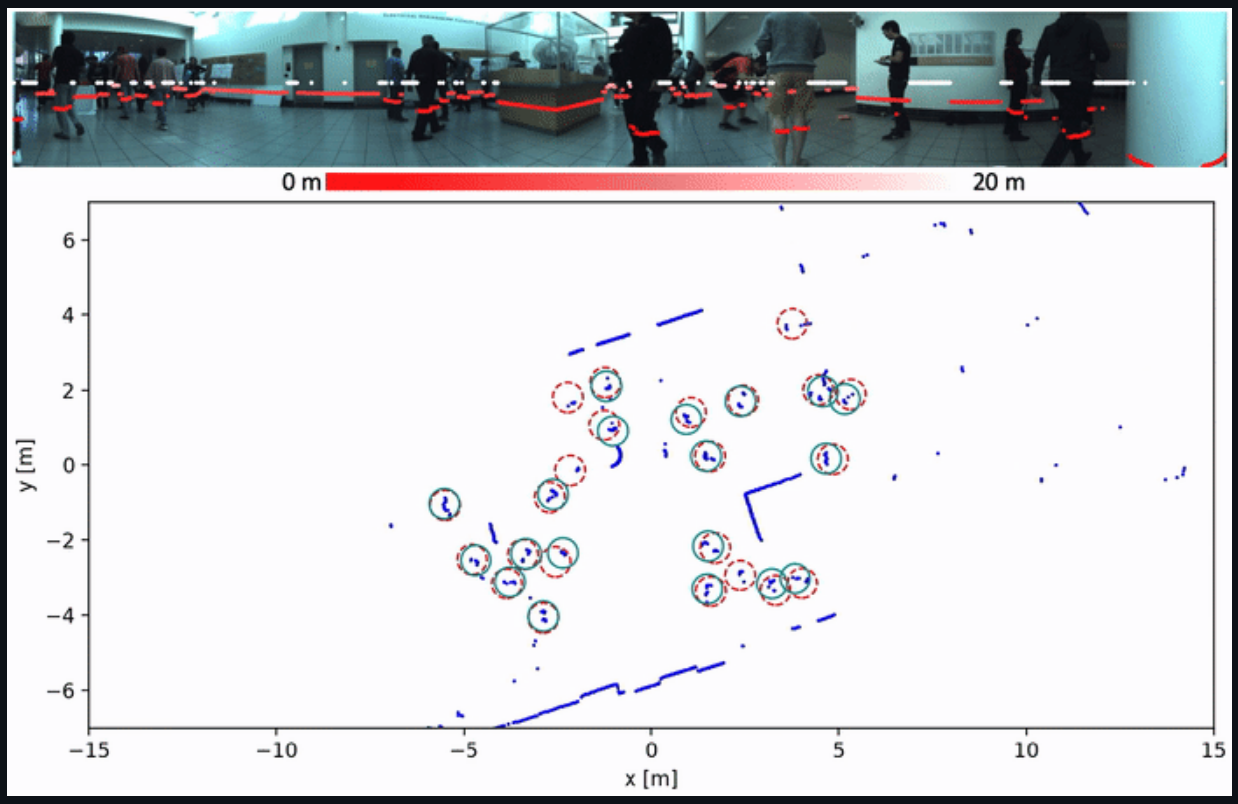
\includegraphics[scale=0.27]{./7_KI/Abbildungen/personen_erkennung_1.png}
        \caption{Symbolfoto Personenerkennung \cite{VisualComputingInstitute2021}}
    \end{minipage}
    \hfill
    \begin{minipage}[b]{0.45\textwidth}
        \centering
        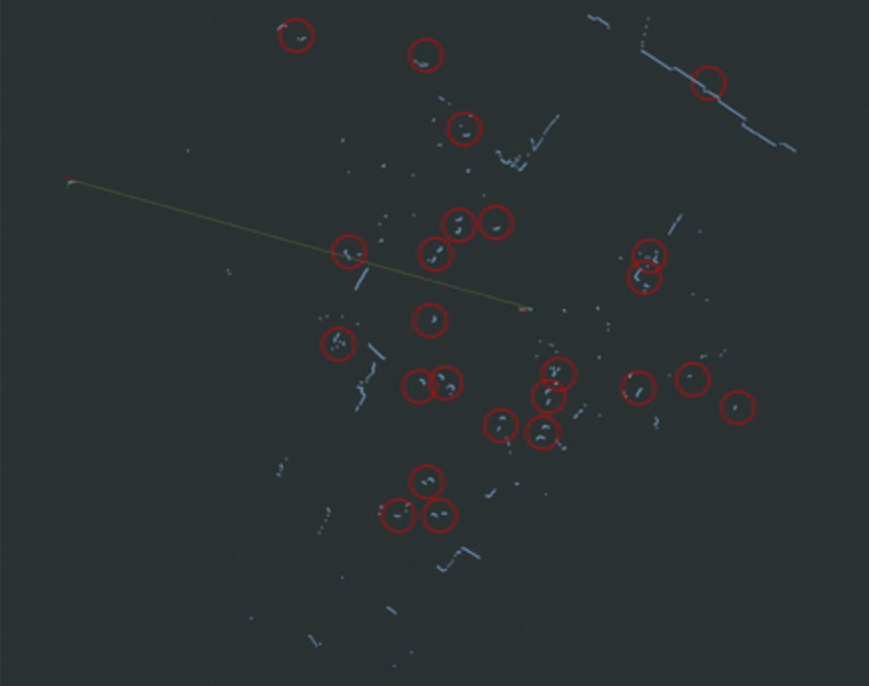
\includegraphics[scale=0.33]{./7_KI/Abbildungen/personen_erkennung_2.png}
        \caption{Symbolfoto Personenerkennung \cite{VisualComputingInstitute2021}}
    \end{minipage}
\end{figure}
\paragraph{Objekterkennung}

Die Objekterkennung ist der erste Schritt des Prozesses, bei dem die KI darauf trainiert wird, Objekte in einem Bild zu identifizieren. Durch den Einsatz von Convolutional Neural Networks (CNNs) werden Merkmale extrahiert und Muster erkannt, welche nicht der normalen Kartenumgebung entsprechen. Sobald ein Objekt erkannt wird, speichert das System die Position und das Bild des erkannten Objekts, um sp�ter darauf zugreifen zu k�nnen.

\paragraph{Objektklassifizierung}
		\begin{figure}[H]
    \centering
        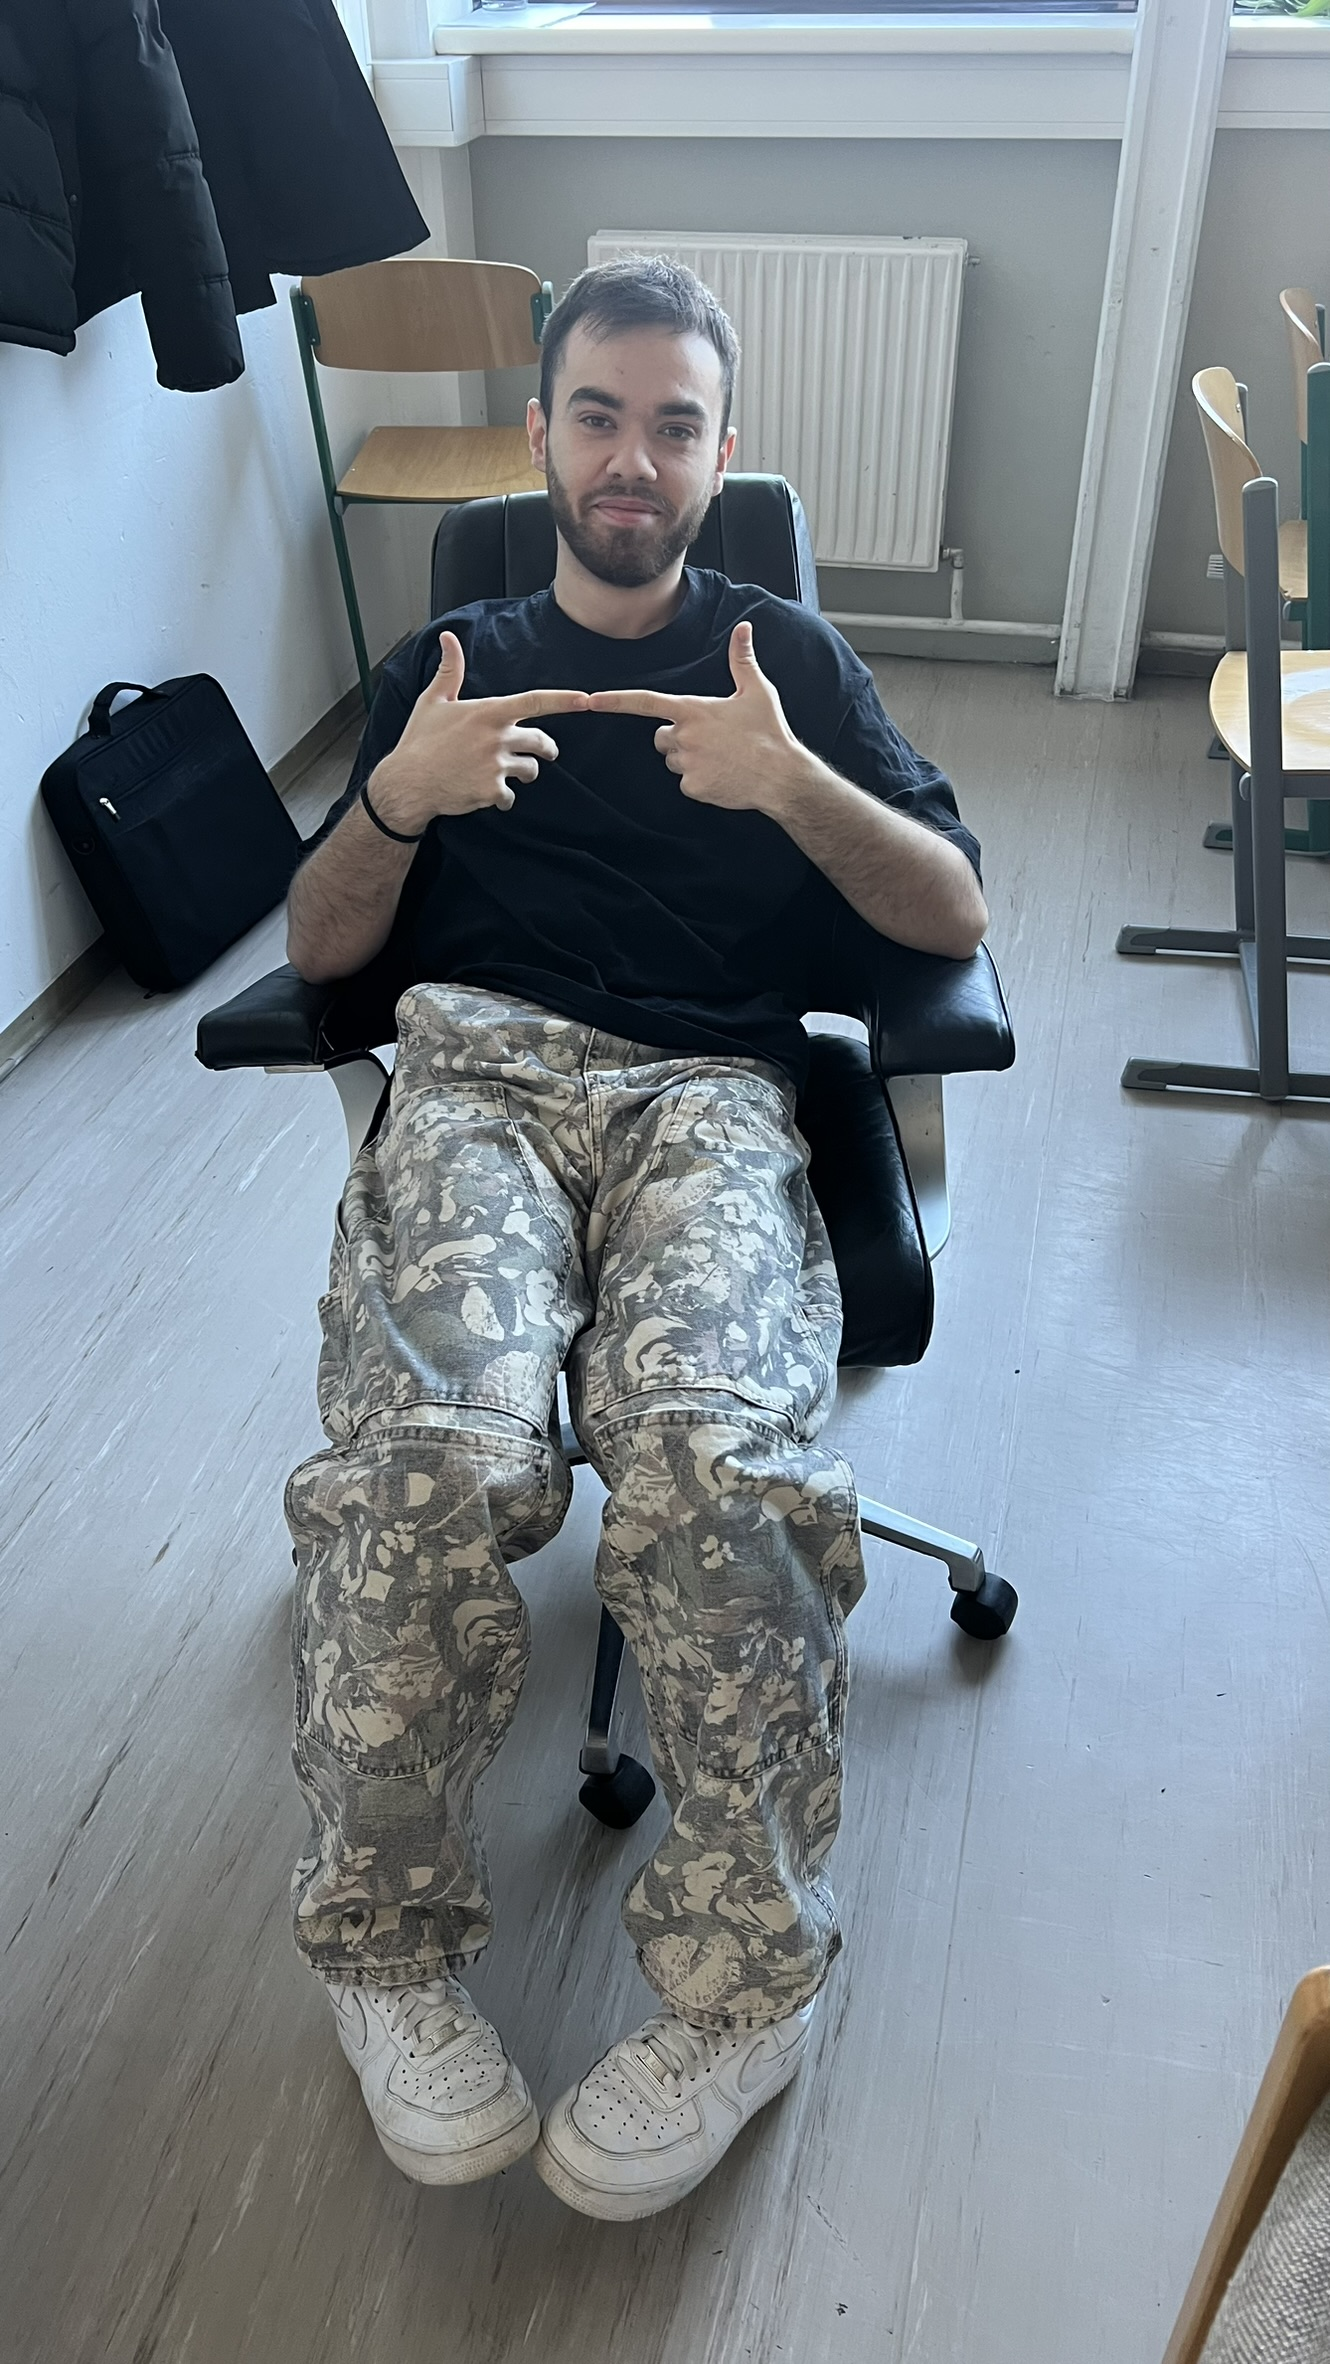
\includegraphics[scale=0.3]{./7_KI/Abbildungen/IMG_3103.JPEG}
        \caption{Symbolfoto einer Person im R�umlichen Verh�ltnis} 
\end{figure}
Nachdem die Position eines erkannten Objekts gespeichert wurde, erfolgt die Klassifizierung dieses Objekts. In diesem Schritt wird die KI darauf trainiert, das erkannte Objekt richtig zu identifizieren, z. B., ob es sich um eine Person handelt oder um ein anderes Objekt. Basierend auf der Klassifizierung werden entsprechende Ma�nahmen ergriffen.

\paragraph{Bereichszuweisung und Sicherheitszonen}

Wenn das erkannte Objekt als Person klassifiziert wird, zeichnet das System eine Sicherheitszone um die gespeicherte Position der Person. Diese Zone markiert den Bereich, der f�r Fahrzeuge oder andere Objekte nicht befahren werden darf, um die Sicherheit der erkannten Personen zu gew�hrleisten. Dies ist besonders wichtig in Anwendungen wie autonomen Fahrzeugen oder Robotern, um Kollisionen zu vermeiden und sicher um Personen herum zu navigieren.

\paragraph{Training der KIs}

Ein wesentlicher Bestandteil des Prozesses ist das kontinuierliche Training der KI-Modelle. Durch die Bereitstellung von Trainingsdaten und die Verwendung von Methoden wie Transfer Learning k�nnen die Modelle verbessert und an neue Umgebungen oder Szenarien angepasst werden. Dies erm�glicht es der KI, genauere und zuverl�ssigere Ergebnisse zu liefern und sich an verschiedene Bedingungen anzupassen.
	
	\fancyfoot[C]{G�rel}
\section{Nutzung von Nodes in ROS}

Die Integration von Programmen in ROS erfordert die Verwendung von Konfigurations- und Launch-Dateien. Diese Dateien legen die Rahmenbedingungen f�r den Betrieb des ROS-Systems fest, konfigurieren die verschiedenen Komponenten und starten die erforderlichen ROS-Knoten. Diese Dateien sind �blicherweise im \texttt{catkin\_ws/src/(node)}-Verzeichnis des ROS-Arbeitsbereichs zu finden.

\paragraph{Konfigurationsdateien}

Um zum Beispiel den Google Cartographer zu verwenden, m�ssen Konfigurationsdateien erstellt werden, die die Parameter f�r den SLAM-Prozess festlegen. Die \texttt{athena\_config.lua}-Datei im Verzeichnis \texttt{cartographer\_ros/configuration\_files} definiert grundlegende Einstellungen.

\paragraph{ROS-Launch-Datei vorbereiten}

Die ROS-Launch-Datei dient dazu, die erforderlichen ROS-Knoten zu starten und die Konfiguration f�r den Google Cartographer bereitzustellen. In der Launch-Datei werden Parameter wie der URDF des Roboters, die Konfiguration der Sensoren und die Pfadangaben zu den Konfigurationsdateien festgelegt. Anschlie�end werden die ROS-Knoten gestartet, darunter der \texttt{robot\_state\_publisher} f�r das URDF, der \texttt{ydlidar\_ros\_driver\_node} f�r den Lidar-Sensor, statische Transformationsknoten und schlie�lich der \texttt{cartographer\_node} f�r den Google Cartographer selbst.

\paragraph{Konfiguration der \texttt{athena\_config.lua}-Datei}

Die \texttt{athena\_config.lua}-Datei enth�lt grundlegende Einstellungen f�r den Cartographer, darunter die Zuordnung von Frame-Namen, die Verwendung von Sensordaten, die Definition von Trajektorien und die Konfiguration des SLAM-Prozesses. Hier werden Parameter wie die Anzahl der Laser-Scans, die L�nge von fehlenden Datenstrahlen, die Verwendung von IMU-Daten und die Scan-Matching-Parameter festgelegt.

\paragraph{Ausf�hren der ROS-Launch-Datei}

Sobald die Konfigurationsdateien und die ROS-Launch-Datei vorbereitet sind, kann der Google Cartographer gestartet werden. 
Beim start ist folgende reihenfolge zu beachten.

\lstset{style=Konsole}
\begin{lstlisting}[language=bash, caption={Konsole 1:}, 
label={code:konsole_1}]
cd catkin_ws
source install_isolated/setup.bash #Sollte eigentlich im bash script automatisch gemacht werden
roscore #Startet den ROS dienst, dieser ist unter anderem f�r den Nachrichtenaustausch verantwortlich
\end{lstlisting}
\begin{lstlisting}[language=bash, caption={Konsole 2:}, 
label={code:konsole_2}]
cd Documents\GitHub\Athena-LattePanda-Code\python #Startet den IMU publisher
python3 publisher.py
\end{lstlisting}
\begin{lstlisting}[language=bash, caption={Konsole 3:}, 
label={code:konsole_3}]
cd catkin_ws
source install_isolated/setup.bash #Sollte eigentlich im bash script automatisch gemacht werden
roscore														#Startet den ROS dienst, dieser ist unter anderem f�r den Nachrichtenaustausch verantwortlich
roslaunch cartographer_ros athena.launch	#Startet den Cartographer dienst
\end{lstlisting}
\begin{lstlisting}[language=bash, caption={Konsole 4:}, 
label={code:konsole_4}]
rosrun rviz rviz	#Startet rviz zur visualisierung des Systems und der Karte
\end{lstlisting}





%% Ergebnisse %%%%%%%%%%%%%%%%%%%%%%%%%%%%%%%%%%%%%%%%%%%%%%%
\newpage
\fancyfoot[C]{Gürel}
\chapter{Ergebnisse und Ausblick}

Das Projekt hat bedeutende Fortschritte gemacht, wobei verschiedene Teams erfolgreich an ihren jeweiligen Aufgaben gearbeitet haben. Die Teamleitung und Entwicklung des elektronischen Aufbaus, einschließlich des Kabelbaums und des Antriebssystems, wurden erfolgreich abgeschlossen. Ebenso wurde die Softwareentwicklung für den Mikrocontroller sowie der 3D-Druck der Bauteile erfolgreich durchgeführt.

Die Finanzierung des Projekts wurde abgeschlossen, und die Benutzeroberflächen sowie das Webdesign wurden erstellt und müssen nun integriert werden. Der mechanische Aufbau, das Design und der Aufbau des Antriebsstrangs, der Aufhängung, der Lenkung und der Karosserie wurden erfolgreich fertiggestellt, ebenso wie die Fertigung und der Zusammenbau der mechanischen Bauteile.

Bezüglich der Herausforderungen gab es Probleme mit der Spannungsversorgung aufgrund qualitativ minderwertiger Komponenten, was wiederholt zu Defekten an Sensoren führte. Lieferzeiten und Bestelldauern einiger Komponenten stellten ebenfalls Hindernisse dar. Ein Kurzschluss auf der Platine war ebenfalls ein Problem, das angegangen werden musste.

Für die Zukunft steht die Fertigstellung der Integration von Finanzierung, Benutzeroberflächen und Webdesign sowie die Entwicklung des ROS-Systems und die Umsetzung von Pathfinding, Personenerkennung und Steuerung des Fahrzeugs an. Mit diesen Schritten werden wir das Projekt abschließen und die gesteckten Ziele erreichen.




%%%%%%%%%%%%%%%%%%%%%%%%%%%%%%%%%%%%%%%%%%%%%%%%%%%%%%%%%%%%%
%% LITERATUR UND ANDERE VERZEICHNISSE
%%%%%%%%%%%%%%%%%%%%%%%%%%%%%%%%%%%%%%%%%%%%%%%%%%%%%%%%%%%%%
\newpage
\pagenumbering{Roman}
%% Ein kleiner Abstand zu den Kapiteln im Inhaltsverzeichnis (toc)
\addtocontents{toc}{\protect\vspace*{\baselineskip}}

%%%%%%%%%%%%%%%%%%%%%%%%%%%%%%%%%%%%%%%%%%%%%%%%%%%%%%%%%%%%%
%% LITERATUR UND ANDERE VERZEICHNISSE
%%%%%%%%%%%%%%%%%%%%%%%%%%%%%%%%%%%%%%%%%%%%%%%%%%%%%%%%%%%%%
%% Ein kleiner Abstand zu den Kapiteln im Inhaltsverzeichnis (toc)
\addtocontents{toc}{\protect\vspace*{\baselineskip}}

%% Literaturverzeichnis
\bibliographystyle{plain}
\bibliography{literatur}


%% Abbildungsverzeichnis
\clearpage
\addcontentsline{toc}{chapter}{Abbildungsverzeichnis}
\listoffigures

%% Tabellenverzeichnis
\clearpage
\addcontentsline{toc}{chapter}{Tabellenverzeichnis}
\listoftables



%%%%%%%%%%%%%%%%%%%%%%%%%%%%%%%%%%%%%%%%%%%%%%%%%%%%%%%%%%%%%
%% ANH�NGE
%%%%%%%%%%%%%%%%%%%%%%%%%%%%%%%%%%%%%%%%%%%%%%%%%%%%%%%%%%%%%
\appendix
%% ==> Schreiben Sie hier Ihren Text oder f�gen Sie externe Dateien ein.

%\input{Dateiname} %Eine Datei 'Dateiname.tex' wird hierf�r ben�tigt.


\end{document}

